  \documentclass[twoside=false, %  doppelseitiger Druck
    DIV=15,% DIV Faktor für Satzspiegelberechnung, sie Doku zu KOMA Script
    BCOR=15mm, % Bindekorrektur
    chapterprefix=false,
    headinclude=true,
    footinclude=false,
    pagesize,%         write pagesize to DVI or PDF
    fontsize=11pt,%             use this font size
    paper=a4,%          use ISO A4
    bibliography=totoc,%         write bibliography-chapter to table of contents
    index=totoc,%         write index-chapter to table of contents
    cleardoublepage=plain,% \cleardoublepage generates pages with pagestyle empty
     headings=big,%       A4/B5
    listof=flat,%        improved list of tables
    numbers=noenddot
  ]{scrbook}

\usepackage[utf8]{inputenc}
\usepackage{makeidx}
\usepackage{amsfonts}
\usepackage[slantedGreek,sc]{mathpazo}  % Schriftart Palatino
% \usepackage{lmodern}    % statt mathpazo, falls CM Fonts verwendet werden sollen
%\usepackage{mathptmx}    % statt mathpazo, falls Times  verwendet werden soll
\usepackage[scaled=.95]{helvet}
\usepackage{courier}
\usepackage[T1]{fontenc}
\usepackage{textcomp}
\usepackage{amsmath}            % standard math notation (vectors/sets/...)
\usepackage{bm}        % standard math notation (fonts)
\usepackage{fixmath}        % standard math notation (fonts)
\usepackage{graphicx}
\usepackage[facing=yes]{floatrow}       % mehrere Gleitobjekte nebeneinander/caption neben Bild/Tabelle
\usepackage[labelfont=bf,sf,font=small,labelsep=space,format=plain]{caption}
\usepackage{subcaption}
\usepackage{scrlayer-scrpage}
% \usepackage{pstool}  % einbinden falls psfrag verwendet werden soll
\usepackage{epstopdf}
\usepackage[ngerman]{babel}
\usepackage{ellipsis}  % Korrigiert den Weißraum um Auslassungspunkte
\usepackage{microtype}  % optischer Randausgleich etc.
\usepackage{enumitem}
\usepackage{xcolor}         % z.B. für schattierte Boxen
\usepackage{framed}			% shaded Umgebung
\usepackage{longtable} % for 'longtable' environment
\usepackage{pdflscape}
\usepackage{multirow}
\usepackage{hhline}
\definecolor{shadecolor}{gray}{.85}%

% Links im PDF
\usepackage[colorlinks=false,
            pdfborder={0 0 0},
            breaklinks=true]
            {hyperref}


%\typearea[current]{calc}


% Einstellungen für Bild-/Tabellenbeschriftung neben dem Bild
\floatsetup[figure]{capbesideposition={inside,top}}
\floatsetup[table]{capbesideposition={inside,top},style=plaintop}
\renewfloatcommand{fcapside}{figure}[\capbeside][\FBwidth]
\newfloatcommand{tcapside}{table}[\capbeside][\FBwidth]


\selectlanguage{ngerman}


\deffootnote{1em}{1em}{%
 \makebox[1em][l]{\thefootnotemark}}

\makeindex

\newcommand{\real}{\mathord{\mathrm{I\!R}}}

\newlist{questions}{enumerate}{2}
\setlist[questions,1]{label=RQ\arabic*.,ref=RQ\arabic*}
\setlist[questions,2]{label=(\alph*),ref=\thequestionsi(\alph*)}

\begin{document}
\selectlanguage{ngerman}
\def\figdir{figures}
\def\tabledir{tables}

\frontmatter

\pagestyle{scrplain}
\pagestyle{empty}

\begin{titlepage}

\sffamily

\raggedleft

\vspace*{-2cm}


\includegraphics{\figdir/logo-th-rosenheim-2019_master_quer_2c.eps}

\vfill

\centering
\LARGE
% \vspace*{\fill}
%-----------
Fakultät für Informatik  \vspace{0.5cm}\\
\Large
Studiengang Software- und Systems-Engineering

\vspace{2cm}

\LARGE

Erkennung von Design Patterns in Quellcode durch Machine Learning

\vspace{2cm}

\Large
Master Thesis

\vspace{1.5cm}


\Large
von

\vspace{0.5cm}

%\vspace*{\fill}

\LARGE
Mehmet Aslan \vspace{1cm}

\vspace{1cm}

\flushleft
 \Large
\vspace*{\fill}

%-----------
\begin{tabbing}
Datum der Abgabe: \= 18.02.2024 \kill
Datum der Abgabe: \> 18.02.2024 \\
Erstprüfer: \> Prof.\ Dr.\ Marcel Tilly\\
Zweitprüfer: \> Prof.\ Dr.\ Kai Höfig
\end{tabbing}
%-----------

\end{titlepage}

\cleardoubleemptypage

{
\large
\thispagestyle{empty}
\vspace*{\fill}

\noindent
\textsc{Eigenständigkeitserklärung / Declaration of Originality}

\medskip

\noindent
Hiermit bestätige ich, dass ich die vorliegende Arbeit selbständig verfasst und keine anderen als die angegebenen Hilfsmittel benutzt habe. Die Stellen der Arbeit, die dem Wortlaut oder dem Sinn nach anderen Werken (dazu zählen auch Internetquellen) entnommen sind, wurden unter Angabe der Quelle kenntlich gemacht.

\medskip

\textit{I declare that I have authored this thesis independently, that I have not used other than the declared sources / resources, and that I have explicitly marked all material which has been quoted either literally or by content from the used sources.}

\bigskip

\noindent
München, den 18.02.2024

\vspace*{2cm}

\noindent
Mehmet Aslan
}

%%% Local Variables: 
%%% mode: latex
%%% TeX-master: "d"
%%% End: 

\cleardoubleemptypage
\chapter*{Kurzfassung}
\thispagestyle{empty}

Design Patterns oder Entwurfsmuster sind in der Software-Entwicklung gängige Lösungsansätze für wiederkehrende Probleme.
Von Software-Entwicklern werden diese eingesetzt, um Probleme in der Implementierung oder in der Software-Architektur zu lösen, deren Lösungsweg bereits bekannt sind und für die jeweilige Situation abgeändert werden. Die wohl bekanntesten Design Patterns sind die 23 Entwurfsmuster nach Gamma et al.
Im weiteren Verlauf der Software-Entwicklung sind die eingesetzten Entwurfsmuster aufgrund iterativer Änderungen und steigender Komplexität im Quellcode nicht mehr einfach wiederzufinden.
Deswegen liegt der Fokus dieser Masterthesis auf der Etablierung eines Prozesses, welcher mit Machine Learning in der Lage ist, Design Pattern im Quellcode zu erkennen.

Das Ziel dieser Arbeit ist es, die Entwurfsmuster Singleton, Observer, Command und Adapter zu identifizieren. Im Kontext dieser Arbeit werden diese als Strukturen definiert, die in Summe von Rollen dargestellt werden.
Jedes dieser Rollen übernimmt im Kontext des jeweiligen Design Patterns unterschiedliche Aufgaben und Verantwortungen.
Dazu wird ein Klassifizierer trainiert, welches Rollen innerhalb dieser Entwurfsmuster durch Code-Metriken erkennt.
Anhand der Klassifikation der Rollen wird im finalen Schritt ein Übereinstimmungswert berechnet, der angibt, mit welcher Zuversicht es sich hierbei um das jeweilige Entwurfsmuster handelt.
Zum Schluss wird die Klassifikationsleistung der hier vorgestellten Methode anhand der Metriken \textit{Precision}, \textit{Recall} und \textit{f1} evaluiert. 

\bigskip

\noindent
Schlagworte: Software-Entwicklung, Machine Learning, Design Patterns 


\cleardoubleemptypage

\pagestyle{scrplain}
\pagenumbering{roman}
% ---------------------------------------------------
% D-TOC.TEX zur Verwendung mit TEXPART
% (an eigene Gegebenheiten anzupassen)
% ---------------------------------------------------
%
\tableofcontents
\clearpage
\listoffigures
\clearpage
\listoftables
\cleardoublepage


\pagestyle{scrheadings}


\addtokomafont{caption}{\small}

\mainmatter

\chapter{Motivation}
\section{Einführung in Design Patterns}

Entwurfsmuster oder auf Englisch `Design Patterns' sind bewährte Lösungsansätze für wiederkehrende Probleme, die bei der Konzeption der Software-Architektur oder während der Implementierung der Software
eingesetzt werden kann. Dabei dienen diese Entwurfsmuster als eine Art Blaupause, die es Software-Entwicklern ermöglicht, erprobte Lösungsstrategien für häufig auftretende Probleme in der Software-Entwicklung anzuwenden.
Durch den Einsatz von etablierten Entwurfsmustern können Software-Entwickler für die Software bei korrekter Anwendung unter anderem erhöhte Wartbarkeit, Wiederverwendbarkeit von Komponenten, Verständlichkeit und Skalierbarkeit ermöglichen das wiederum in qualitativ besserer Software resultiert.
Dabei sollte beachtet werden, dass Design Patterns als Vorlage zu betrachten sind. Je nach Einsatzgebiet muss die Anwendung des Entwurfsmusters evaluiert und für den konkreten Fall individualisiert werden.
Deshalb existiert keine universelle anwendbare Iteration eines Design Patterns, die unabhängig von Anwendungskontext eingesetzt werden kann. Dies resultiert in variierenden Anwendung von Entwurfsmustern abhängig von jeweiligem Einsatzgebiet.
Im weiteren Entwicklungszyklus der Software werden durch neue oder geänderte Anforderungen bereits eingesetzte Implementierungen von Entwurfsmustern modifiziert, entfernt oder neue werden hinzugefügt.
Währenddessen besteht die Gelegenheit, dass durch mangelnder Dokumentation oder anderer Gründe die Entscheidungen, weshalb Entwurfsmuster so eingesetzt sind wie es eingesetzt worden, verloren gehen.
Dadurch besteht die Gefahr, dass angewendete Design Patterns im weiteren Verlauf derer Entwicklung nicht mehr wiederzuerkennen sind. Aus diesem Grund ist die Etablierung eines Prozesses von Vorteil, das in der Lage ist,
Implementierungen von Entwurfsmustern aus einem Software-System zu extrahieren und dieses konkret benennen. Vor allem der Einsatz von Maschine Learning für die Klasszifierung ist hier vorteilhaft, wodurch das Potenzial besteht, vorher nicht gesehene Implementierung von Design Patterns zu erkennen.
Durch solch einen Prozess können durch die Erkennung von eingesetzten Entwurfsmustern auf konkrete und verlorenen gegangene Design-Entscheidungen zurückgeschlossen werden, welche zukünftige Design-Entscheidungen für das Software-System beeinflussen können. 
Der Fokus dieser Arbeit besteht daran, solch ein Prozess zu etablieren, welches für ein gegebenes Set von Quellcode-Dateien mithilfe von Maschine Learning einem potenziellen Entwurfsmuster zuzuteilen.  

\newpage

\section{Untersuchungsfragen}

Das Ziel dieser Arbeit besteht aus der Etablierung eines Prozesses, womit durch Einsatz von Maschine Learning für ein Set von Quellcode-Dateien ein Design Pattern zuzuordnen.
Hierfür dienen eine Menge an Quelldateien als Eingabe für den Prozess und durch phasenweiser Transformationen und Bearbeitungen sollen ein möglichst passendes aus dem in Kontext dieser Arbeit betrachteten Entwurfsmusters zugeordnet werden.
Um solch ein Prozess zu entwickeln, werden in Kontext dieser Arbeit folgende Fragen beantwortet:

\begin{questions}
    \item Welche Design Patterns werden berücksichtigt?
    \item Was für ein Datensatz eignet sich für solch ein Prozess?
    \item Wonach wird exakt klassifiziert?
    \item Welche Merkmale, die aus Quellcode-Dateien extrahierbar sind, eignen sich für Klasszifierung durch Maschine Learning Modelle?  
    \item Welche Klassifizierer eignen sich?
    \item Wie ist das Endresultat zu beurteilen?
\end{questions}

\section{Übersicht des Prozesses}



\chapter{Literaturrecherche}
\section{Design Patterns in der Software-Entwicklung}

Entwurfsmuster definieren gängige Lösungsblaupausen für häufig auftretende Probleme in Software-Entwicklung, vor allem in der Design-Phase der Architektur des Software-Systems
als auch während der konkreten Implementierung. Jedoch sind diese als Schablone zu verstehen, die für den jeweiligen Einsatzfall angepasst werden müssen.
Ein Werk, dass das Verständnis von Design Patterns für das objektorientierte Programmieren maßgeblich geprägt, ist das von Gamma et al. verfasste Arbeit "Design Patterns: Elements of Reusable Object-Oriented Software".
In diesem wird ein Katalog von 23 Entwurfsmustern definiert, welche in drei Kategorien aufgeteilt. Dieser Katalog wird von Software-Entwicklern als "Gang of Four" Entwurfsmuster bezeichnet. Gamma et al. definieren folgende Elemente für die Identifikation eines Entwurfsmusters:\cite[S. 3]{gamma1994design}

\begin{itemize}
    \item \textbf{Pattern Name}: Der Name des Entwurfsmusters beschreibt in wenigen Worten, welches das zu lösende Problem, die Lösung und welche Folgen dessen Einsatz mit sich bringt. Durch die Einführung eines Bezeichners wird eine Schicht der Abstraktion hinzugefügt, welches das Verständnis und Dokumentation des Design Patterns vereinfacht.
    \item \textbf{Problem}: Das Problem beschreibt, wo das Entwurfsmuster angewendet werden soll. Dabei kann es sich um ein konkretes Entwurfsproblem, Klassen- oder Objektstrukturen oder eine Liste von Bedingungen darstellen, die zu erfüllen sind.
    \item \textbf{Solution}: Das Lösungselement beschreibt die Beziehungen, Verantwortlichkeiten und Zusammenarbeit der einzelnen Elemente, die die Struktur des Design Patterns definieren. Dabei werden diese Elemente in Objekte und Klassen, die die Grundbausteine der objektorientierten Programmierung repräsentieren, aufgeteilt und deren Interaktionen miteinander stellen die Verantwortlichkeiten und Beziehungen dar.
    \item \textbf{Consequences}: Die Folgen diskutieren, wie der Einsatz des betrachteten Entwurfsmusters sich auf das Software-System einwirkt und welche Vor- und Nachteile dadurch resultieren. Diese beeinflussen unter anderem die Zeit- und Speicherkomplexität, Erweiterbarkeit, Flexibilität und Portabilität des Software-Systems.
\end{itemize}

Im Kontext dieser Arbeit werden zu klassifizierende Strukturen, die potenziell einem Design Pattern zugeordnet werden können, als Mikroarchitekturen bezeichnet, die aus einer Menge von interagierenden Komponenten bestehen, denen je eine Rolle zugewiesen wird. Die jeweilige Rolle beschreibt, welche Funktionalität und Verantwortung diese im Kontext der Mikroarchitektur übernimmt und wie diese mit anderen Komponenten interagiert.
Als Komponenten mit Rollen werden hier konkrete bzw\. abstrakte Klassen oder Schnittstellen definiert, die erforderte Rolle im Rahmen der Mikroarchitektur erfüllen.

In weiteren Verlauf dieser Sektion werden die drei erwähnten Entwurfsmusterkategorien erläutert und zu dem werden im Kontext dieser Arbeit betrachte spezifische Design Pattern genauer betrachtet.

\newpage

\section{Design Pattern Katalog}

\subsection{Creational Design Patterns}

Die Kategorie der Creational Design Patterns oder Erzeugungsentwurfsmuster beschäftigt sich mit der Abstraktion des Prozesses der Initialisierung\cite[S. 81]{gamma1994design}. Entwurfsmuster dieser Kategorie fokussieren sich auf die Unabhängigkeit wie Objekte erstellt, zusammengesetzt und repräsentiert werden.
Die Entwurfsmuster dieser Kategorie mit Fokus auf Klassen nutzen den Mechanismus der Vererbung, um zu beeinflussen, wie Komponenten instantiiert werden, während dahingegen Design Patterns mit einem Fokus auf Objekten die Instantiierung auf andere Objekte delegieren.
Creational Design Patterns werden dann bedeutend, wenn mit steigender Komplexität des Software-Systems sich von Vererbung distanziert wird und die Komposition aus einzelnen definierten Objekt mehr an Bedeutung gewinnt\cite[S. 81]{gamma1994design}. Dabei wird das Verhalten einer Komponente auf eine Menge von einzelnen kleinere Objekten delegiert und durch Zusammensetzung innerhalb der Komponente und deren Interaktion das erwünschte Verhalten erzeugt.
Dadruch wird die Instantiierung von Software-Komponenten komplexer, da die Instantiierung von mehreren Objekten koordiniert werden muss. Creational Design Patterns liefern hierbei Hilfestellung, weil die exakte Komposition der konkreten Objekte, die Teil der zu instantiierenden Komponente sind, und der exakte Prozess der Instantiierung im Inneren des Entwurfsmusters verborgen werden. Nach außen hin sind dahingegen nur die Schnittstellen sichtbar, die die Komponente zur Verfügung stellt, während dessen interene Logik die Ausführung auf andere Objekte delegiert.
Im Kontext dieser Arbeit werden folgende Entwurfsmuster aus der Kategorie der Creational Design Patterns betrachtet:

\subsubsection{Singleton}

\begin{figure}[h]
    \centering
    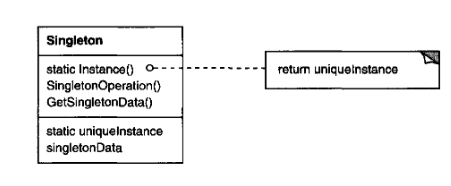
\includegraphics{figures/singleton.png}
    \caption{UML-Diagramm für Singleton}
    \label{fig:singleton}
\end{figure}

Die Abbildung~\ref{fig:singleton} zeigt den strukturellen Aufbau eines Singletons~\cite[S. 127]{gamma1994design}.
Dabei kann dieser nach Gamma et al. wie folgt beschrieben werden:

\begin{description}
    \item[Problem] \hfill \\
    \begin{itemize}
        \item Exakt eine Instanz der Klasse zur selben Zeit verfügbar; Zugreifbar zu Klienten durch bekannten Zugangspunkt
        \item Einzige Instanz erweiterbar durch Vererbung; Nutzbarkeit der Subklasse ohne Veränderung des Quellcodes auf Klientenseite
    \end{itemize}
    \item[Solution] \hfill
    \begin{itemize}
        \item   Zugriff auf Singleton-Instanz durch Instance-Operation
    \end{itemize}
    \item[Roles] \hfill \\
    \begin{description}
        \item[Singleton] \hfill \\
        \begin{itemize}
            \item Definiert eine Instance-Operation für Zugriff auf einzige Instanz
            \item Mögliche selbstsändige Instanziierung
        \end{itemize}
    \end{description}
    \item[Consequences]  \hfill 
    \begin{itemize}
        \item Kontrollierter Zugriff auf Instanz
        \item Mögliche Verfeinerung der Operationen und Repräsentation durch Vererbung
        \item Nachträgliche Änderung der Anzahl der Instanzen 
    \end{itemize}
\end{description}

\subsubsection{Factory Method}

\begin{figure}[h]
    \centering
    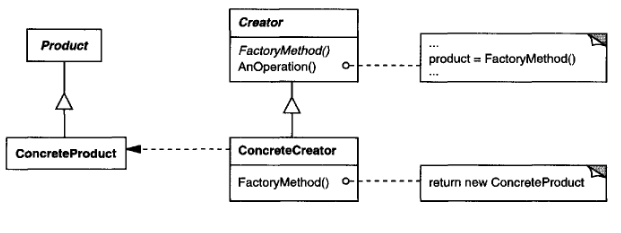
\includegraphics[scale=0.8]{figures/factory.png}
    \caption{UML-Diagramm für Factory Method}
    \label{fig:factory}
\end{figure}

Abbildung~\ref{fig:factory} beschreibt exemplarisch die Struktur einer Factory Method~\cite[S. 108]{gamma1994design}.
Diese wird nach Gamma et al. auf folgende Art und Weise beschrieben:

\begin{description}
    \item[Problem] \hfill 
    \begin{itemize}
        \item Eine Klasse kann die Klasse der Objekte, die es instantiiert, im Voraus nicht erahnen
        \item Eine Klasse verlangt, dass ihre Unterklassen die von ihr erstellten Objekte spezifizieren
        \item Klassen delegieren die Instantiierung von Objekten an Helferklassen
    \end{itemize}

    \item[Role] \hfill
    \begin{description}
        \item[Product] \hfill
        \begin{itemize}
            \item definiert die Schnittstelle der Objekte, die die Factory-Methode erzeugt
        \end{itemize}
        \item[ConcreteProduct] \hfill
        \begin{itemize}
            \item implementiert die Schnittstelle Product
        \end{itemize}
        \item[Creator] \hfill 
        \begin{itemize}
            \item deklariert die Factory-Methode, die ein Objekt vom Typ Product zurückgibt
            \item kann auch eine Standardimplementierung der Factory-Methode definieren, die die ein Standard ConcreteProduct-Objekt zurückgibt
            \item kann die Factory-Methode aufrufen, um ein Product-Objekt zu erzeugen
        \end{itemize}
        \item[ConcreteCreator] \hfill
        \begin{itemize}
            \item überschreibt die Factory-Methode, um eine Instanz eines ConcreteProduct zurückzugeben
        \end{itemize}
    \end{description}

    \item[Consequences] \hfill
    \begin{itemize}
        \item Eliminierung der Bindung an applikationsspezifische Klassen; Interaktion durch Product-Schnittstelle
        \item Flexibilität bei der Instanziierung von Objekten.
    \end{itemize}

\end{description}


%%TODO: Add concrete design patterns
\subsubsection{Structural Design Patterns}

Structural Design Patterns oder Strukturentwurfsmuster fokussieren sich darauf, wie einzelne Klassen und Objekte zusammengesetzt werden können, um größere Strukturen zu erzeugen\cite[S. 137]{gamma1994design}.
Entwurfsmuster dieser Kategorie sind vorteilhaft, wenn unabhängig voneinander entwickelte Klassen oder Objekte aus verschiedenen Bibliotheken oder Frameworks miteinander interagieren müssen.
Anstatt konkrete Implementierung und Schnittstellen zu nutzen, bedienen sich Structural Design Patterns der Komposition aus Objekten, um neue Funktionalitäten zur Verfügung zu stellen\cite[S. 137]{gamma1994design}.
Die dadurch gewonnene Flexibilität ermöglicht das Ändern der Zusammensetzung des Objektes dynamisch zu der Laufzeit, welches mit statischer Komposition durch Klassen nicht möglich ist.\cite[S. 137]{gamma1994design}.
Im Kontext dieser Arbeit werden folgende Entwurfsmuster aus der Kategorie der Structural Design Patterns betrachtet:

\subsubsection{Adapter}

\begin{figure}[h]
    \centering
    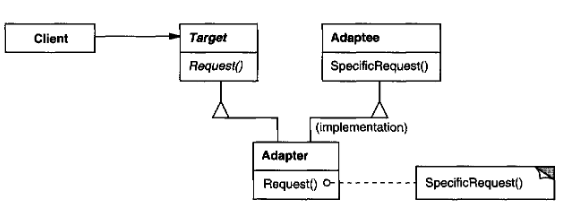
\includegraphics[scale=0.75]{figures/adapter.png}
    \caption{UML-Diagramm für Adapter}
    \label{fig:adapter}
\end{figure}

Abbildung~\ref{fig:adapter} zeigt die Struktur des Adapter-Entwurfsmusters. 
Dabei wird ein Adapter nach Gamma et al. wie gefolgt beschrieben~\cite[S. 141]{gamma1994design}:


.\begin{description}
    \item[Problem] \hfill
    \begin{itemize}
        \item Eine existierende Klasse soll genutzt werden; die Schnittstelle der Klasse stimmen mit der gebrauchten nicht überein
        \item Recyclebare Klasse, die mit unabhängigen Klassen kooperiert
    \end{itemize}
    \item[Roles] \hfill
    \begin{description}
        \item[Target] \hfill
        \begin{itemize}
            \item definiert domain-spezifische Schnittstelle für das Nutzen durch Clients
        \end{itemize}
        \item[Client] \hfill 
        \begin{itemize}
            \item kollaboriert mit Objekten, die Target-Schnittstelle implementieren
        \end{itemize}
        \item[Adaptee] \hfill 
        \begin{itemize}
            \item definiert ein bereits existierende Schnittstelle, worauf Adapter abgepasst wird
        \end{itemize}
        \item[Adapter] \hfill 
        \begin{itemize}
            \item adoptiert die Schnittstelle von Adaptee zu Target-Schnittstelle
        \end{itemize}
    \end{description}
    \item[Consequences] \hfill 
        \begin{itemize}
            \item Adoptierung von Adaptee zu Target-Schnittstelle durch konkrete Adapter-Klasse
            \item Adapter überschreibt Verhalten von Adaptee-Klasse, da Adapter Subklasse von Adaptee 
        \end{itemize}
\end{description}

\pagebreak

\subsubsection{Behavioral Design Patterns}

Behavioral Design Patterns oder Verhaltensentwurfsmuster konzentrieren sich auf Algorithmen und der Zuweisung von Verantwortlichkeiten zwischen Objekten\cite[S. 221]{gamma1994design}.
Dabei wird nicht nur Struktur der Entwurfsmuster betrachtet, sondern auch die Kommunikation und Interaktion der Objekte, die Teil des Entwurfsmusters sind. Charakteristisch für Design Patterns dieser Kategorie ist der Fokus auf Verknüpfung der einzelnen Teilobjekte des Entwurfsmusters,
anstatt des Kontrollflusses, welcher zur Laufzeit schwer nachvollziehbar sein kann~\cite[S. 221]{gamma1994design}.
Im Kontext dieser Arbeit werden folgende Entwurfsmuster aus der Kategorie der Behavioral Design Patterns betrachtet:

\subsubsection{Command}

\begin{figure}[h]
    \centering
    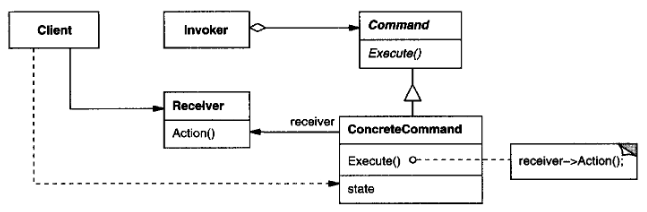
\includegraphics[scale=0.75]{figures/command.png}
    \caption{UML-Diagramm für Command}
    \label{fig:command}
\end{figure}

Abbildung~\ref{fig:command} zeigt die Struktur des Adapter-Entwurfsmusters. 
Dabei wird Command nach Gamma et al. wie gefolgt beschrieben~\cite[S. 236]{gamma1994design}:

\begin{description}
    \item[Problem] \hfill 
    \begin{itemize}
        \item Kapsulierung von Aktion durch parametrisierbare Objekte
        \item Spezifizierung, Abwarten und Ausführung von Aktionen zu verschiedenen Zeiten;
        \item Option für Undo; ausgeführte Aktion wird rückgängig gemacht
    \end{itemize}
    \item[Roles] \hfill
    \begin{description}
        \item[Command] \hfill
        \begin{itemize}
            \item deklariert eine Schnittstelle für das Ausführen von Operationen
        \end{itemize}
        \item[ConcreteCommand] \hfill
        \begin{itemize}
            \item definiert eine Bindung zwischen einem Receiver und einer Aktion
            \item implementiert Execute-Methode durch Ausführen des korrespondierenden Operationen auf Seite von Receiver
        \end{itemize}
        \item[Invoker] \hfill
        \begin{itemize}
            \item initialisiert die Ausführung eines Commands
        \end{itemize}
        \item[Receiver] \hfill
        \begin{itemize}
            \item Empfänger von Commands
            \item Wissen, wie empfangene Commands auszuführen sind  
        \end{itemize}
    \end{description}
    \item[Consequences] \hfill
    \begin{itemize}
        \item Entkoppelung zwischen Objekt, welches Operation initialisiert, und Objekt, das Operation durchführt
        \item Erweiterung von Manipulation von Verhalten von Command-Klassen durch Vererbung
        \item Zusammensetzung von Command-Klassen durch andere Command-Klassen
        \item Erleichtertes Hinzufügen von neuen Command-Klassen
    \end{itemize}
\end{description}

\subsubsection{Observer}

\begin{figure}[h]
    \centering
    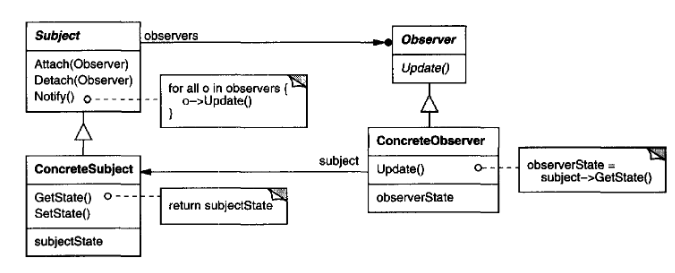
\includegraphics[scale=0.75]{figures/observer.png}
    \caption{UML-Diagramm für Observer}
    \label{fig:observer}
\end{figure}

Die Abbildung~\ref{fig:observer} zeigt den strukturellen Aufbau eines Observers~\cite[S. 293]{gamma1994design}.
Dabei kann dieser nach Gamma et al. wie folgt beschrieben werden:

\begin{description}
    \item[Problem] \hfill 
    \begin{itemize}
        \item Benachrichtigung von Objekten ohne Annahmen über diese
        \item Änderung in einem Objekt erfordert Änderungen in abhängigen Objekten; Kein Wissen wie abhängige Objekte auf Änderung reagieren
    \end{itemize}
    \item[Roles] \hfill
    \begin{description}
        \item[Subject] \hfill 
        \begin{itemize}
            \item Wissen über dessen Observer; beliebige Anzahl an Observern an einem Subject möglich
            \item Schnittstelle für das Hinzufügen und Entfernen von Observern
        \end{itemize}
        \item[Observer] \hfill 
        \begin{itemize}
            \item definiert Schnittstelle für das Reagieren von Änderungen am Subject seitens der abhängigen Objekte
        \end{itemize}
        \item[ConcreteSubject] \hfill 
        \begin{itemize}
            \item implementiert Subject-Schnittstelle
            \item beinhaltet relevanten Zustand von ConcreteObserver-Objekten
            \item Benachrichtigung von dessen Observer-Objekten bei Änderungen am relevanten Zustand
        \end{itemize}
        \item[ConcreteObserver] \hfill 
        \begin{itemize}
            \item hält Referenz zu ConcreteSubject-Objekt
            \item Speichert selbst Zustand; konsistent zu dem von Subject
            \item implementiert Observer-Schnittstelle für das Synchronisieren der Zustände  
        \end{itemize}
    \end{description}
    \item[Consequences]:
    \begin{itemize}
        \item Abstrakte Koppelung zwischen Observer und Subject; Keine Annahmen von Subject über Observer außer Observer-Schnittstelle
        \item Broadcast an Observer; Benachrichtigung aller registrierten Observer
        \item Einspielen von unerwarteten Benachrichtigung 
    \end{itemize}
\end{description}
\section{Herausforderungen und Probleme bei der Erkennung von Design Patterns}

In diesem Abschnitt der Arbeit werden mögliche Herausforderungen diskutiert, die bei dem Entwerfen des Prozesses für die Erkennung von Entwurfsmustern auftreten können. 

\subsection*{Variabilität der Implementierung}

Design Patterns stellen in der Software-Entwicklung bewährte Lösungsmuster für bereits begegnete Herausforderung dar. Aufgrund der abstrakten und wiederverwendbaren Natur der Entwurfsmuster,
muss für diese eine konkrete Implementierung definiert werden, die von dem Einsatzfall, Kontext und anderen Faktoren wie verwendeter Programmiersprache, Bibliotheken und Erfahrungsstand des Software-Entwicklers.
Dadruch, dass jedes Entwurfsmuster einen konzeptionellen Rahmen darstellt und jede Implementierung von nicht statischer Außenfaktoren beeinflusst wird, resultiert dies in einem breiten Spektrum an Implementierungen für ein gegebenes Entwurfsmuster.
Aus diesem Grund ist eine Definition einer starren Definition eines Design Patterns, was als Startpunkt und Referenz für die Erkennung des jeweiligen Entwurfsmusters dienen könnte, nicht möglich. 
Deshalb ist eine definitive Antwort auf die Frage, ob eine betrachte Mikroarchitektur eine Instanz eines Entwurfsmusters, nicht beantwortbar, weshalb die Antwort von automatisierten Prozessen von Design Patterns eher mit einem Wert besteht,
welches die Ähnlichkeit zu einem Design Pattern beschreibt. Um einen zufriedenstellenden Wert für diese Frage zu liefern, bedarf es eines bereiten Spektrums an Implementierungsvariationen als Referenz für die Erkennung.

\subsection*{Steigende Komplexität von Software-Systemen}

Die steigende Komplexität von Software-Systemen stellt eine erhebliche Herausforderung bei der Erkennung von Entwurfsmustern in Entwurfsmustern dar.
Dies ist besonders bei langjährigen Software-Projekten der Fall, an denen über die Zeit konstante Änderungen wegen Wartung und neuen bzw. geänderten Anforderungen unterliegen.
Diese Art von Software-Projekten tendieren dazu, dass mit der Zeit deren Komplexität zunimmt~\cite[S. 7]{Suh-2010}. 
Bei kleineren Software-Projekten mit geringem Umfang und Komplexität sind Entwurfsmuster leichter zu erkennen und zu implementieren.
Dahingegen bei langjährigen Software-Projekten steigt mit wachsender Gesamtkomplexität die Komplexität der angewendeten Entwurfsmuster in deren Quellcode, wodurch die Identifizierung dieser proportional mitsteigt.
Entwurfsmuster werden durch diese Entwicklung weiter modifiziert und angepasst, womit diese von der ursprünglichen leichter zu identifizierbaren Iterationen weiter abweichen. 
Deshalb beinhaltet die Erkennung von Entwurfsmustern nicht nur auf die momentane Iteration, sondern auch die Erfassung derer historischen Evolution und die Entwicklung dieser innerhalb der Codebasis.

\newpage

\subsection*{Iterative Evolution des Quellcodes}

Damit ein Software-System seine Anforderungen im Verlauf dessen Lebenszyklus in einer zufriedenstellenden Art und Weise erfüllen kann, muss dieses adaptieren, um diesen Anforderungen gerecht zu werden~\cite[S. 108]{10.1007/BFb0017737}.
Dies hat zu Folge, dass dessen Quellcode iterativen Änderungen unterliegt. Ursprüngliche Implementierungen in der Codebasis werden analysiert und es wird überprüft, ob diese ihre Aufgaben zufriedenstellend erfüllen oder nicht.
Falls nicht, werden diese so modifiziert, sodass diese Anforderungen auf erwartete Art und Weise erfüllt werden können. Implementierungen von angewandten Design Patterns als Teil des Quellcodes unterliegen ebenfalls dieser Analyse.
Diese werden als Teil des Analyseprozesses genauer betrachtet und werden nach Bedarf modifiziert und angepasst. Diese Entwicklung führt wie das im vorherigen Abschnitt diskutierten Fall, dass Entwurfsmuster von ihrer ursprünglichen leichter zu identifizierbaren
Iteration weiter abweichen und die Erkennung von Entwurfsmustern nicht nur die momentane Implementierung, sondern auch die historische Entwicklung berücksichtigen werden muss. In automatisierten Prozess der Erkennung von Entwurfsmustern kann dieser Aspekt nur bedingt berücksichtigt,
weil das Einschließen der Historie der betrachtenden Implementierung und dessen Kontext in der Codebasis nicht pauschal und in einer allgemeinen Ansicht betrachtet werden kann. 

\subsection*{Mangel an expliziter Dokumentation}

Das Erstellen und Warten von Dokumentation für Software-Systeme ist eine Tätigkeit, die von Software-Entwicklern als wichtig eingestuft wird, jedoch in diese Tätigkeit relativ wenig Zeit investiert wird~\cite[S, 162]{zhi2015cost}.
Dies ist die Folge der Dominanz des agilen Software-Entwicklungsprozesses, in dieser die Verwendung von Zeit und Ressourcen für die Dokumentation eher als Verschwendung betrachtet wird, da diese keinen direkten Mehrwert für die Auslieferung des Software-Produktes an den Endkunden liefert~\cite[S. 159]{zhi2015cost}.
Das dies das Software-System komplett betrifft, sind Design Patterns in dessen Codebasis ebenfalls betroffen. Diese werden meist nicht direkt gekennzeichnet. 
Zwar kann durch Nomenklatur und Kontrollfluss indirekt Rückschlüsse auf die potenziellen Entwurfsmuster abgeleitet werden, jedoch erfordert dies konkretes Fachwissen und Erfahrungen, die nicht von jedem Software-Entwickler erfüllt werden kann.
Bei automatisierten Prozessen für die Erkennung von Entwurfsmustern kann diese berücksichtigt werden, sollte aber nicht als alleiniger Faktor bei dem Identifikationsprozess dienen.\\

Aufgrund der Variation an Implementierungsmöglichkeiten, Änderungen im Quellcode und Mangel an Dokumentation ist die manuelle Identifikation von Entwurfsmustern in Quellcode ein Prozess dar,
in der einen gewissen Grad an Mitdenken erfordert. Im nächsten Abschnitt der Arbeit werden bereits entwickelte Verfahren betrachtet, die das Mitdenken bis zu einem gewissen Grad automatisieren und dieses als Teil des Prozesses mitinludieren.





\section{Maschine Learning}

Der Fokus dieser Arbeit ist die Ermittlung von Design von Quellcode durch die Anwendung von Maschine Learning.
Dieser Teil der Arbeit ist für die Erläuterung von verwendeten Metriken, angewandten Techniken und ausgewählter Klassifizierer gewidmet.

% TODO: \subsection{Terminologie} falls notwendig
\subsection{Metriken für Evaluierung von Modellen}

Um die Leistung eines Klassifizierers zu ermitteln, bedarf es einer Menge an Metriken, womit beurteilt werden, ob der Klassifizierer wie erwartet performt.
In Kontext dieser Aussage wird in der Domäne des Maschine Learnings bekannte Metriken aus dem Bereich der Statistik angewendet.
In diesem Abschnitt wird eine Auswahl von solchen Metriken erläutert, die in der Literaturrecherche als auch in den Sektionen der Methodik und Implementierung erwähnt werden.
Für die Ermittelung der Metriken werden folgende Größen definiert:

\begin{description}
    \item TP (True Positive): Anzahl echt positiver Klassifizierungen
    \item TN (True Negative): Anzahl echt negativer Klassifizierungen
    \item FP (False Postive): Anzahl falsch positiv Klassifizierungen
    \item FN (False Negative): Anzahl falsch negativ Klassifizierungen
\end{description}

Anhand dieser Größen werden folgende Metriken definiert:

\begin{description}
    \item \textit{Accuracy (Genauigkeit)}: Dieser Wert gibt an, wie das Verhältnis zwischen den klassifizierten Beobachtungen zur Gesamtzahl der Beobachtungen ist.
    \\
    \\
    $Accuracy = \frac{\text{Anzahl der korrekten Vorhersagen}}{\text{Gesamtzahl der Vorhersagen}} = \frac{TP+TN}{TP+TN+FP+FN}$

    \item \textit{Precision (Präzision)}: Dieser Wert gibt das Verhältnis an, wie die korrekt positiv klassifizierten Beobachtungen zur Gesamtzahl der als positiv klassifizierten Beobachtungen stehen.
    \\
    \\
    $Precision = \frac{TP}{TP+FP}$

    \item \textit{Recall (Sensitivität)}: : Dies ist das Verhältnis der positiv klassifizierten Beobachtungen zur Gesamtzahl der tatsächlichen positiven Beobachtungen.
    \\
    \\
    $Recall = \frac{TP}{TP+FN}$
    
    \item \textit{ F1-Score}: Der F1-Score ist das harmonische Mittel von Präzision und Recall und gibt ein besseres Maß für die unbalancierten Klassen als die Genauigkeit allein.
    \\
    \\
    $\textit{\text{F1-Score}} = 2 * \frac{Precision * Recall}{Precision + Recall} = \frac{2*TP}{2*TP + FP + FN}$
\end{description}

\pagebreak

\subsection{Validierung und Optimierung von Modellen}

Neben dem Zusammentragen von relevanten Datenpunkte für die Erhebung eines geeigneten Datensatzes ist das Validierung und Optimierung des Maschine Learning Modells eines der relevanten Schritte im gesamten Prozess, 
um damit das Modell dessen Aufgabe möglichst zufriedenstellend erfüllen kann. 
In diesem Teil der Arbeit werden Techniken bzw. Methoden erläutert, die in der Validierungs- oder Optimierungsphase angewendet werden können.


\subsubsection{Kreuzvalidierung von Modellen}
Nach dem Trainieren des Modells für einen Datensatz ist von Interesse, wie das Modell neue unbekannte Datenpunkte umgeht und diese Leistung anhand einer Metrik zu messen.
Dies stellt den Kernpunkt der Validierungsphase dar. Ein naiver Ansatz, die gleiche Menge an Datenpunkten zu verwenden, worauf das Modell in der Trainingsphase trainiert wurde.
Dabei ist jeder Datenpunkt des Datensatzes dem Modell bereits bekannt, wodurch es nicht auf wirklich unbekannte Datenpunkte validiert.
Eine Möglichkeit dem entgegenzukommen ist das Aufteilen des Datensatzes in Trainings- und Validationsdatensatz, wobei meist der Trainingsdatensatz die größere Menge an Datenpunkten zugesprochen wird.
Jedoch besteht hier der Nachteil, das in der Trainingsphase die Datenpunkte in dem Validationsdatensatz wegfallen.
Um diesen Nachteil zu negieren, kann die Technik der Cross Validation oder Kreuzvalidierung angewendet werden.

Hierbei wird zunächst eine natürliche Zahl \textit{n} bestimmt, die angibt, in wie viele gleich große Teile der Datensatz aufgeteilt wird.
Die Trainings- und Validierungsphase wird hierbei zu einem Schritt zusammengefasst und das Modell wird iterativ \textit{n}-Mal trainiert und anhand der vorgegebenen Metrik evaluiert.

\begin{figure}[h]
    \centering
    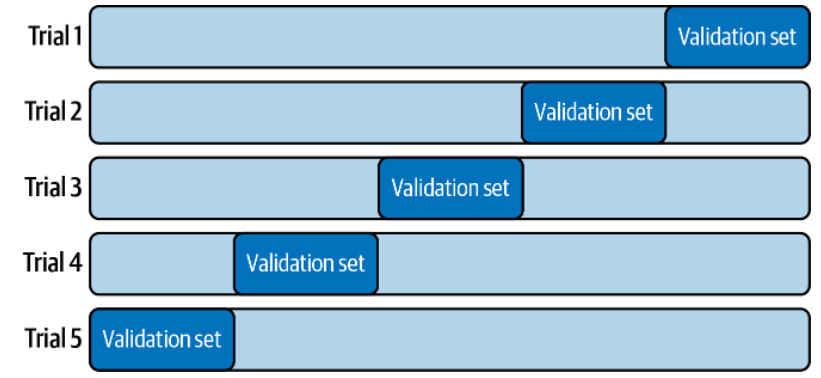
\includegraphics[scale=0.5]{figures/cross_validation}
    \caption{Kreuzvalidierung mit \textit{n} = 5}
    \label{fig:cross_validation}
\end{figure}
Wie aus Abbildung \ref{fig:cross_validation} zu entnehmen ist, wird in der \textit{i}-ten Iteration das $k-i$-te Sektion des Datensatzes für die Validierung und restlichen
für das Training des Modells verwendet. Das Resultat dieser Operation ist abhängig von Implementierung der Kreuzvalidierung die Iteration des Modells mit der besten Evaluation und eine Liste von Werten, die Leistung des Modells in der jeweiligen Iteration angibt.

\pagebreak

\subsubsection*{Optimieren von Modellen durch Hyperparameter-Tuning}
Maschine Learning Modelle können mithilfe von Parametern konfiguriert werden. Dabei wird zwischen zwei Arten von Parametern entschieden: Modellparameter und Hyperparameter.
Modellparameter werden während der Trainingsphase automatisiert direkt durch den Trainingsdatensatz bestimmt und sind nicht von Außen zu manipulieren. Dahingegen bestimmen Hyperparameter unter anderem wie sich das Modell während der Trainingsphase zu verhalten und beeinflussen
dessen Architektur. Jedes Modell definiert hierbei selbst, welche Hyperparameter verfügbar sind. Hyperparameter werden während der Instantiierung des Modells definiert. Die Ermittelung der bestmöglichen Kombinationen an Hyperparametern-Werten ist hilfreich, falls Leistung des Modells nicht den Erwartungen entspricht und das verwendete Datensatz nicht weiter argumentiert werden kann.
Um die Leistung des Modells zu evaluieren, wird wie in der Kreuzvalidierung eine Metrik bestimmt, die Leistung der jetzigen Iterationen zu beurteilen. Das Ziel der Hyperparameter-Optimierung besteht hier darin, eine Kombination an Hyperparametern-Werten zu bestimmen, wodurch die Metrik maximiert bzw. minimiert. 
Dies kann entweder manuell durchgeführt oder es werden Methoden eingesetzt, die dies automatisiert erledigen können. Im Folgendem wird eine Auswahl an automatisierten Strategien aufgelistet und erläutert:

\begin{description}
    \item Random Search/Grid Search: In diesen Methoden werden zunächst Wertebereiche für die jeweiligen Hyperparameter bestimmt. In der Regel wird hierbei eine Menge an diskreten Wertem bestimmt, die der jeweilige Hyperparameter annehmen kann. Jede Permutation der Hyperparameter-Konfiguration wird als eine Zelle in einem Gitter erfasst. 
    Jede besuchte Zelle dient dabei als Konfiguration für eine neue Instanz des Modells, welches im weiteren Verlauf durch Einsatz von Kreuzvalidierung trainiert und evaluiert wird. Das Ergebnis der Evaluation wird vermerkt.
    Bei Random Search wird zufällig bestimmt, welche Zellen besucht werden, während bei Grid Search alle Zellen besucht werden. Das Ergebnis ist die Konfiguration des Modells mit der besten Evaluierung.
    
    \item Bayessche Optimierung: Bei Grid bwz. Random Search wird jede Permutation der Hyperparameter-Werte eine Instanz des Modells trainiert und evaluiert. Unter Umständen kann der Trainingsprozess je nach Modell und Datensatz rechenintensiv, wodurch es lange dauern, bis diese Methoden ein Resultat liefern.
    In solch einem Fall kann das Verfahren der Bayesschen Optimierung angewendet, um die Dauer der Evaluierung zu verkürzen. Im Kern wird das Maschine-Learning Modell als Black Box Funktion interpretiert, welches als Eingabe eine Permutation an Hyperparameter-Werten akzeptiert und der Wert der Zielmetrik für die jeweilige Permutation dient als Rückgabewert der Black Box Funktion.
    Dadurch, dass die Optimierung der Black Box Funktion durch Ableitungsverfahren nicht möglich, wird dieses eine Ersatzfunktion substituiert, welches die Black Box Funktion approximiert.
    Bei der Ersatzfunktion handelt es such um ein probabilistisches Modell, welches genutzt wird, um eine Wahrscheinlichkeitsverteilung über die möglichen Werte der Zielmetrik für verschiedene Kombinationen an Hyperparameter-Werten zu erstellen.
    Die Bayessche Optimierung beginnt typischerweise mit einer zufälligen Auswahl von Hyperparametern, um einige Datenpunkte zu generieren. Diese werden verwendet, um das probabilistische Modell zu initialisieren. Anschließend wird iterativ die Akquisitionsfunktion angewendet, um neue und vielversprechende Hyperparameter-Kombinationen zu identifizieren und zu testen. 
    Diese Funktion bestimmt, welche Permutation am Hyperparameter-Werten auf Basis des jetzigen Standes des probabilistischen Modells als Nächstes bewertet werden soll. 
    Sie balanciert die Exploration unbekannter Bereiche des Hyperparameterraums mit der Exploitation von Bereichen, die voraussichtlich zu besseren Ergebnissen führen.
    Nach jedem Schritt wird das Modell mit den neuen Ergebnissen aktualisiert, was zu einer kontinuierlichen Verbesserung der Schätzungen und Entscheidungen führt. Am Ende der Methode ist die Kombination an Hyperparameter-Werten bekannt, welches für die Zielmetrik das globale Minimum bzw. Maximum als Rückgabewert zurückgibt.

    \item Tree-structured Parzen Estimators (TPE): Bei TPEs handelt es sich um einen speziellen Anwendungsfall der Bayesschen Optimierung. Anstatt eine Wahrscheinlichkeitsverteilung für die Kombination an Hyperparameter-Werten zu verwenden, wird diese in zwei aufgeteilt:
    eine für Kombinationen, die zu besseren Werten für die Zielmetrik führen ("gute Verteilung") und eine für solche, die zu schlechteren Ergebnissen führen ("schlechte Verteilung"). Wie bei der normalen Bayesschen Optimierung wird eine Aquisefunktion eingesetzt, um zu bestimmen, welche Kombination an Hyperparameter-Werten als Nächstes evaluiert werden soll.
    Hierbei basiert die Akquisitionsfunktion bei TPE auf das Verhältnis der Dichten dieser beiden Verteilungen. Durch den Einsatz von Parzen Estimatoren werden für beide Wahrscheinlichkeitsverteilungen Dichtefunktionen approximiert, wodurch die Dichten in Akquisitionsfunktion bestimmt werden können.
    Sie wählt die nächste zu evaluierende Hyperparameter-Kombination, indem sie Bereiche bevorzugt, in denen das Verhältnis der Dichte der "guten" Verteilung zur Dichte der "schlechten" Verteilung hoch ist.
    Wie in der normalen Bayesschen Optimierung wird das probabilistische Modell iterativ mit neuen Werten aktualisiert, um ein globales Minimum bzw. Maximum der Black Box Funktion zu ermitteln.

\end{description}

\pagebreak
%%TODO: Add references from literature

\subsection{Betrachtete Klassifizierer}
Für die Bestimmung eines Design Patterns wird eine Menge an Rollen bestimmt, die die Submuster innerhalb des jeweiligen Entwurfsmusters erfüllen.
Die Bestimmung der Rollen für einzelne Submuster fällt in dem Bereich des Maschine-Learnings in den Bereich der Klassifikation. Im Sinne dieser werden in diesem Abschnitt der Arbeit eine Auswahl von Klassifizierern betrachtet und erläutert,
die im Kontext dieser Arbeit in Anbetracht gezogen werden.

\subsubsection*{Support Vector Maschines}

Support Vector Mashines oder SVMs sind überwachte Maschine-Learning Modelle, die sowohl für Regressions- als auch für Klassifikationsaufgaben einsetzbar ist. Die Datenpunkte werden in einen \textit{n}-dimensionalen Raum abgebildet, wobei \textit{n} die Anzahl der Features der Datenpunkte beschreibt.
Bei der Klassifizierung trennen SVMs den Raum der Datenpunkte in verschiedene Zonen. Jede Zone entspricht einem Label, zu welchen die Datenpunkte in der jeweiligen Zone zugeordnet werden. Die Grenzen der einzelnen Zonen werden durch Hyperplanes beschrieben. Das Ziel ist, diese Hyperplanes so zu bestimmen,
sodass die Datenpunkte möglichst distinkt einer Zone zugeordnet werden.

\begin{figure}[h]
    \centering
    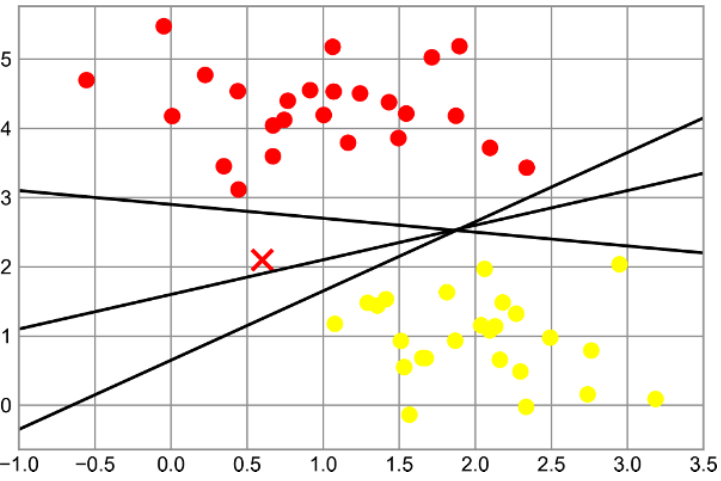
\includegraphics[scale=0.5]{figures/support_vector_new_point.png}
    \caption{Grafische Darstellung einer SVM im zwei-dimensionalen Raum}
    \label{fig:svm_graphic}
\end{figure}

Abbildung \ref{fig:svm_graphic} grafisch, wie eine SVM funktioniert. Punkte sind die Datenpunkte des Datensatzes und die Farben der Punkte die Klasse, in der die Punkte eingeordnet sind.
Die Linien beschreiben die mögliche Hyperplanes, womit Grenzen zwischen den Klassen determiniert wird. Das Kreuz zeigt einen neuen Datenpunkt, der zu klassifizieren ist. Mit diesem neuen Datenpunkt stellt sich die Frage, welche der drei möglichen Hyperplanes zu wählen ist, um die Datenpunkte möglichst distinkt einer Klasse zuzuordnen.

\pagebreak

\begin{figure}[h]
    \centering
    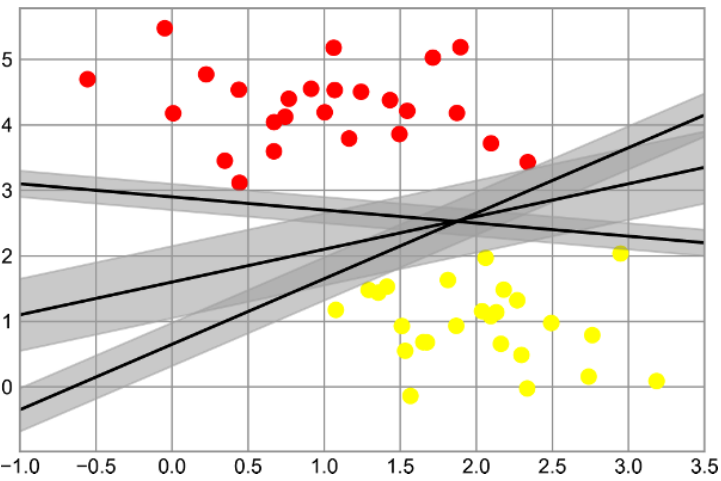
\includegraphics[scale=0.5]{figures/support_vector_maschine_margins.png}
    \caption{Hyperplanes mit Margen}
    \label{fig:svm_margins}
\end{figure}

Wie in Abbildung \ref{fig:svm_margins} zu sehen ist, wird für jede Hyperplane die Marge zwischen der Hyperplane und der Datenpunkte und den nächsten Datenpunkten bestimmt.
Die Hyperplane mit der größten Marge, die mit der größten Distanz zwischen sich und den nächsten Datenpunkten, wird als finale Hyperplane für die Grenzbildung zwischen den Klassen gewählt. Im Falle von Abbildung \ref{fig:svm_margins}
ist dies mittlere von den drei Kandidaten. Mit jedem neuen Datenpunkt wird währed Trainings wird die ideale Hyperplane neu bestimmt.
Jedoch stellt sich die Frage, wie mit Datensätzen umzugehen, die nicht durch lineare Hyperplanes in Klassen aufgeteilt werden.

\pagebreak

\begin{figure}[h]
    \centering
    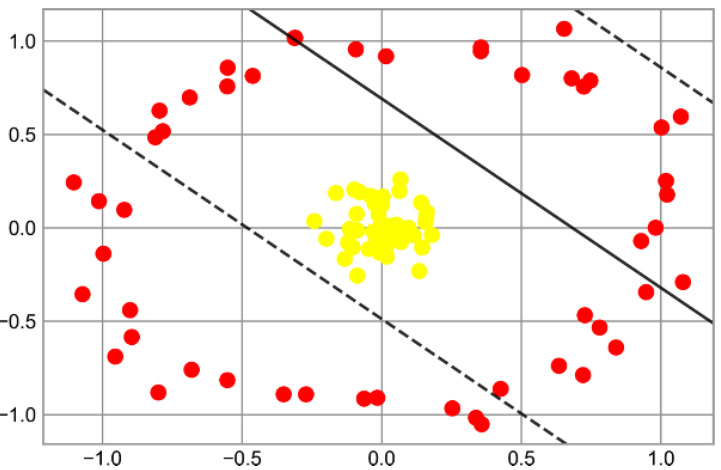
\includegraphics[scale=0.5]{figures/svm_non_linear.png}
    \caption{Nicht mögliche Einteilung durch lineare Hyperplanes}
    \label{fig:svm_non_linear}
\end{figure}


Abbildung \ref{fig:svm_non_linear} zeigt einen Datensatz, dessen Datenpunkte nicht distinkt durch lineare Hyperplanes zugeordnet werden können. Um trotzdem lineare Hyerplanes zu bilden,
wird der bei SVMs Kernel verwendet. Bei dem Kernel Trick handelt es sich um eine Funktion, die den Datensatz in einen Raum mit einer höheren Dimension projektiert.
Durch die Projektion in einem Raum mit einer höheren Dimension ist es möglich, lineare Hyperplanes zu bestimmen.
Diese Funktion werden als Kernel bezeichnet und werden bei der Instantiierung des Modells als Hyperparameter mitgegeben.

\begin{figure}[h]
    \centering
    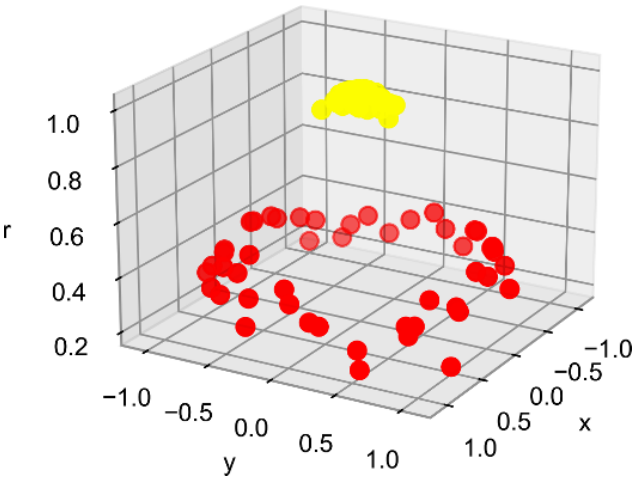
\includegraphics[scale=0.5]{figures/svm_kernel_transformation.png}
    \caption{Transformierter Datensatz aus Abbildung \ref{fig:svm_non_linear} durch RBF}
    \label{fig:svm_transformed}
\end{figure}

Abbildung \ref{fig:svm_transformed} zeigt, wie durch Anwendung des Radial-Basis-Function Kernel, das den ursprünglich zwei-dimensionalen Raum auf ein drei-dimensionales projektiert wird.
Durch die Transformation kann nun eine Hyperplane als Ebene bestimmt werden, wodurch die Klassifikation ermöglicht wird.

\pagebreak

\subsubsection*{k-Nearest Neighbor Classifier}

k-Nearest Neighbors Classifier oder KNN kann wie die SVM für Regressions- als auch für Klassifikationsprobleme eingesetzt werden. Dabei wird bei KNN unter der Annahme agiert, dass ähnliche Datenpunkte in der Nähe zueinander sind.
Der Hyperparameter k definiert die Anzahl der nächsten Nachbarn, die verwendet werden, um den neu eingefügten Datenpunkt eine Klasse zuzuordnen. Um die k nächsten benachbarten Datenpunkte zu identifizieren, ist ein Maß erforderlich, welches die Distanz zwischen diesen beschreibt. 
Folgende Größen können als Metrik für die Distanz verwendet werden:

\begin{description}
    \item Euklidische Distanz ist die Länge des Liniensegmentes zwischen den beiden Punkten im euklidischen Raum.
    \\
    \begin{math}
        d_{euclidean} (P, Q)= \sqrt{(p_1 - q_1)^2 + (p_2 + q_2)^2 + \ldots + (p_n - q_n)^2}
        \\
        \\
        \text{mit}
        \\
        \\
         P = (p_1, p_2, \ldots, p_n)
         \\
         Q = (q_1, q_2, \ldots, q_n)
    \end{math}
    
    \item Manhattan Distanz ist die Summe der absoluten Differenz zwischen den Komponenten der Punkte.
    \\
    \begin{math}
        d_{manhatten} (P, Q) = |p_1 - q_1| + |p_2 - q_2| + \ldots + |p_n - q_n|
        \\
        \\
        \text{mit}
        \\
        \\
         P = (p_1, p_2, \ldots, p_n)
         \\
         Q = (q_1, q_2, \ldots, q_n) 
    \end{math}
    \item Minkowski Distanz ist eine allgemeinere Metrik, um die Distanz zwischen zwei Punkten im n-dimensionalen Raum zu ermitteln.
    \\
    \begin{math}
        d_{minkowski}(P, Q) = (|p_1 - q_1|^p + \ldots + |p_n - q_n|^p)^\frac{1}{p}
        \\
        \\
        \text{mit}
        \\
        \\
         P = (p_1, p_2, \ldots, p_n)
         \\
         Q = (q_1, q_2, \ldots, q_n)
         \\
         p = \text{Typ der zu kalkulierenden Distanz ($p = 1$ --> Manhatten Distanz, $p = 2$ --> Euklidische Distanz)} 
    \end{math}
\end{description}
Die Klassifizierung des neuen Datenpunktes erfolgt im Kontext der k nächsten benachbarten Datenpunkte. Die Klasse, welche am häufigsten in den k benachbarten Punkten vorkommt, wird dem neuen Datenpunkt zugewiesen.

\subsubsection*{Random Forest Classifier}
%%TODO
\section{Angewandte Ansätze für die Erkennung von Design Patterns}

Bei der Erkennung von Design Patterns in Quellcode wurden verschiedene Verfahren entwickelt, die auf unterschiedlichen Methoden beruhen, um das gesetzte Ziel zu erreichen.
Yarahmadi et al.~führten in ihrer Arbeit eine Untersuchung über die Methoden, die angewandt worden sind, um Design Patterns in Quellcode zu erkennen, durch und kategorisierten diese~\cite[S. 5805]{yarahmadi2020design}.

\begin{figure}[h]
    \centering
    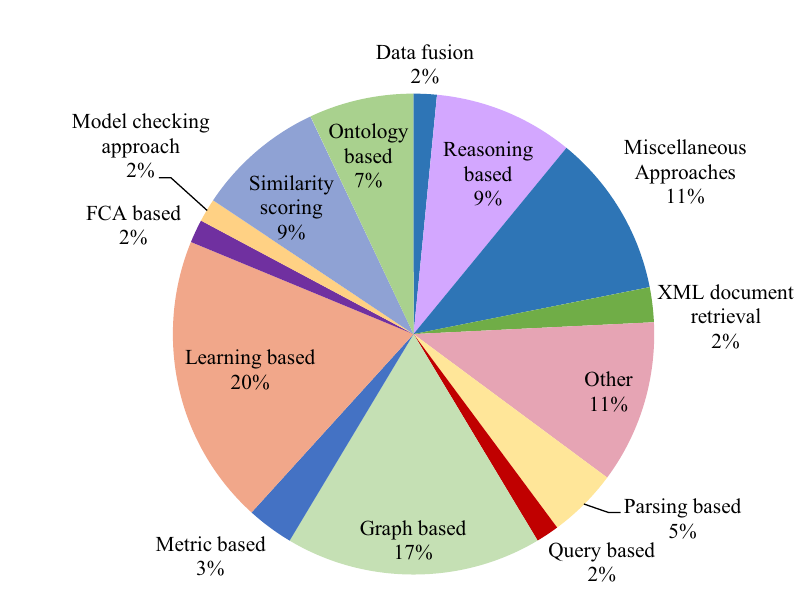
\includegraphics[scale=0.5]{figures/approches_distribution.png}
    \caption{Verteilung der Kategorien der Ansätze für die Erkennung von Design Patterns in Quellcode}
    \label{fig:approach_dist}
\end{figure}

Wie aus Figur~\ref{fig:approach_dist} zu entnehmen ist, wurden die entwickelten Prozesse von Yarahmadi et al. auf eine begrenzte Menge an Kategorien eingestuft.
In dieser Sektion der Arbeit werden die vier größten Kategorien aus Figur~\ref{fig:approach_dist} genauer erläutert und es werden exemplarische Arbeiten diskutiert, die zu der jeweilige Kategorie zugeordnet werden.

\subsection{Graphen-basierende Ansätze}

Die Methodik der Reduktion stellt in der Berechenbarkeitstheorie einen Ansatz dar, um Lösungswege für neue unbekannte Probleme zu entwickeln. Dabei wird durch einen Algorithmus das unbekannte Problem in ein bereits gelöstes Problem, dessen Lösungsweg schon vorhanden ist, umgewandelt.
In Graphen-basierenden Methoden für die Erkennung von Design Pattern in Quellcode wird diese angewendet, um Quellcode in Graphen zu transformieren und diese Graphen werden als Eingabe für diverse Graphenalgorithmen verwendet.

\pagebreak

Formell betrachtet ist ein Graph definiert als~\cite[S. 9]{Siu1998IntroductionTG}:
\begin{align*}
& \text{G} = \{V(G), E(G)\}
&\\
&\text{mit}
&\\
&G : \text{der zu betrachtende Graph}\\
&V (G): \text{Nicht leere Menge von Knoten in G}\\
&E (G): \text{Menge an ungeordneten Tupeln von distinkten Elementen von V (G)}
\end{align*}

Der Quellcode selbst ist als roher Text zu betrachten, welcher verschiedene Entitäten wie Klassen, Objekte und Schnittstellen beinhaltet und definiert, wie diese miteinander interagieren. Als Graph $G$ werden die Entitäten aus dem Quellcode als Knoten $V (G)$ und 
die Relationen und Interaktionen wie Vererbung oder Methodenaufrufe werden als Kanten $E (G)$ dargestellt.
Hierbei stellt Unified Modeling Language (UML) eine in der Software-Entwicklung verbreitete Modellierungssprache dar und definiert verschiedene Arten von Graphen, um Software und andere Systeme zu modellieren.
Die Diagramme aus der UML-Domäne werden in diesem Kontext als Graphen aufgefasst, da diese aus einer Menge aus Kanten und Konten bestehen und anhand der obigen Definition als Graphen interpretiert werden können.
Eine Diagrammart aus der Domäne, welches eingesetzt wird, um objektorientierte (OO) Software-Systeme zu modellieren, sind Klassendiagramme.
Klassendiagramme beschreiben, wie Klassen und deren Relation zueinander im Kontext des Paradigmas der objektorientierten Programmierung aufgefasst werden.
Pradhan et al.\ nutzen Klassendiagramme als Eingabe für ihre entworfene Methode und generieren diese für das zu analysierende Software-System und Implementierungen von Entwurfsmustern, die als Referenz genutzt werden~\cite[S. 2]{7346680}.
Diese werden als gerichtete Graphen erfasst, wobei die Klassen als Knoten und die Assoziation wie Vererbung zwischen diesen als Kanten aufgefasst werden. Zusätzlich werden die Kanten je nach Art der Assoziation unterschiedlich gewichtet~\cite[S. 2]{7346680}.
Im weiteren Verlauf werden mögliche Kandidaten aus dem Graphen des Software-Systems extrahiert. Durch den Einsatz der Graphenisomorphie wird zwischen den Subgraphen des Software-Systems und den Referenzgraphen der Entwurfsmuster die normalisierten Kreuzrelation als das Maß der Übereinstimmung berechnet~\cite[S. 3]{7346680}.
Graphenisomorphie beschreibt, ob zwei Graphen strukturell identisch sind, sodass jede Kante des einen Graphen einer Kante im anderen Graphen entspricht und umgekehrt~\cite[S. 10]{Siu1998IntroductionTG}. Die normalisierte Kreuzrelation ist ein Maß, dessen Wertebereich zwischen 0.0 und 1.0 definiert ist.
Je näher der Wert an der oberen Grenze 1.0, desto identischer sind die zwei Graphen. 
Zu der Evaluierung des Prozesses wurden vier Open-Source-Software-Systeme hergezogen, aus welchen fünf existierende Entwurfsmuster zu erkennen sind~\cite[S. 6]{7346680}. Dabei wurde von Pradhan et al. dokumentiert, ob ein Entwurfsmuster komplett oder partiell im Quellcode entdeckt wurde.
Nach eigener Auswertung von Pradhan et al. wurden die als Referenz genommene Implementierung der Design Patterns mehrfach komplett als auch partiell in der Codebasis der zu dem Test hergezogenen Software-Systeme identifiziert~\cite[S. 6]{7346680}.

\pagebreak

In ihrer Arbeit verfolgen Dongjin et al. ebenfalls die Erkennung von Entwurfsmustern der strukturellen Kategorie in Quellcode durch den Einsatz von Graphen. In Kontext dieser werden wie im vorherigen Verfahren beschriebenen Klassendiagramme als gerichtete gewichtete Graphen eingesetzt.
Entitäten wie Klassen, Objekte oder Schnittstellen werden als Knoten und die Assoziation der Entitäten wie Vererbung als gerichtete gewichtete Kanten des Graphen repräsentiert~\cite[S. 582]{6649882}.
Zudem werden Referenzimplementierungen der zu identifizierenden Entwurfsmuster in gewichtete Klassendiagramme transformiert und innerhalb dieser werden Submuster definiert, die in Summe das Entwurfsmuster repräsentieren~\cite[S. 580]{6649882}.

\begin{figure}[h]
    \centering
    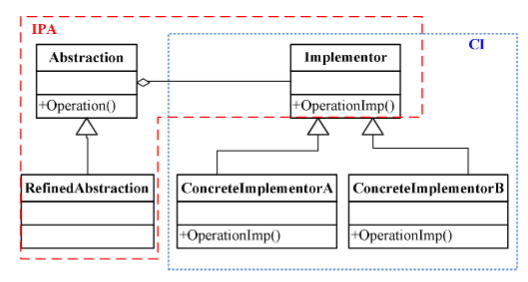
\includegraphics[scale=0.75]{figures/struture_bridge.png}
    \caption{Referenzklassendiagramm des Bridge Patterns mit Submustern}
    \label{fig:structure_bridge}
\end{figure}

Beispielhaft spiegelt die Abbildung \ref{fig:structure_bridge} von Dongjin et al. das definierte Referenzklassendiagramm das Bridge Pattern wieder. Innerhalb dieses Klassendiagramms werden die Submuster \textbf{IPA} und \textbf{CI} festgelegt. Wie von der Abbildung \ref{fig:structure_bridge} zu entnehmen ist, bestehen die Submuster aus einzelnen Entitäten und deren Assoziationen.
Innerhalb der Klassendiagramme des Quellcodes, welches als Eingabe dient, wird nach solchen Submustern durch Einsatz von Graphenisomorphie gesucht~\cite[S. 584]{6649882}. Im weiteren Verlauf werden identifizierte, relevante Submuster zu einer Kandidatenstruktur verschmolzen. Dabei ist anzumerken, dass nur die Submuster, die im betrachtenden Entwurfsmuster vorkommen, in der Verschmelzung involviert sind.
Als finaler Schritt werden durch Analyse des Verhaltensmusters der Kandidatenstrukturen falsch positiv identifizierte Instanzen herausgefiltert~\cite[S. 584]{6649882}. Quellcode aus vier Open-Source-Software-Systemen dient als Eingabe für dieses Verfahren~\cite[S. 585]{6649882}. 
Zu Evaluierung der Resultate der Methodik wird die Metrik der \textit{Precision} verwendet. Dabei wird das Verhältnis zwischen der Anzahl der positiv falschen identifizierten Instanzen zu der Summe der Anzahl der positiv falsch und falsch positiv klassifizierten Instanzen gebildet~\cite[S. 585]{6649882}. Je höher diese ist, desto besser ist das Ergebnis einzustufen.
Nach eigenständiger Evaluierung von Dongjin et al. wird für alle Software-Systeme für alle betrachten strukturellen Entwurfsmuster eine hohe Rate der \textit{Precision} ermittelt~\cite[S. 586]{6649882}.

%TODO: Add this file:///home/memi/Downloads/Yu,%20Dongjin_%20Zhang,%20Yanyan_%20Ge,%20Jianlin_%20Wu,%20Wei%20-%20[IEEE%202013%20IEEE%2037th%20Annual%20Computer%20Software%20and%20Applications%20Conference%20(COMPSAC)%20-%20Kyoto,%20Japan%20(2013.07.22-2013.07.26)]%20201%20(2013,%20IEEE)%20[10.1109_COMPSAC.2013.92]%20-%20libge.pdf

\pagebreak

\subsection{Machine Learning Ansätze}

Mit der ersten öffentlich zugänglichen Version des Open Source Machine Learning Frameworks TensorFlow am 9. November 2015 wurde der Zugang für praktisch angewandtes Machine Learning für Software-Entwickler erleichtert. Durch TensorFlow wird eine Abstraktionsschicht für das Entwerfen, Trainieren und den Betrieb von Machine Learning Modellen eingeführt. Der vereinfachte Einsatz resultiert mit der Anwendung von Machine Learning in Produkten und in der Forschung. Dies ist auch der Fall für die Erkennung von Design Patterns in Quellcode.
Wie aus Abbildung~\ref{fig:approach_dist} zu entnehmen ist, stellen nach der Untersuchung von Yarahmadi et al. Verfahren, die Machine Learning einsetzen, einen signifikanten Teil dar.
Im Kontext dieser Aussage werden in diesem Abschnitt ausgewählte Verfahren erläutert, die Machine Learning als Teil des Erkennungsprozesses anwenden.
Der Fokus in dieser Sektion liegt neben den angewandten Modellen für die Klassifikation auf dem Format der Eingabe, in der die Quellcode-Dateien für die Klassifikation transformiert werden.

Eine Möglichkeit, um Entitäten aus dem Quellcode wie Klassen oder Schnittstellen und deren Assoziation darzustellen, ist die Darstellung als Klassendiagramme aus der UML-Domäne.
In ihrer Methodik nutzen Wang et al. UML-Klassendiagramme als Grundlage und modifizieren diese mit der Inkorporation von Farb- und Symbolcodierungen. Dieses Format benennen Wang et al. \textit{Colored UML}~\cite[S. 6]{app12178718}.

\begin{figure}[h]
    \centering
    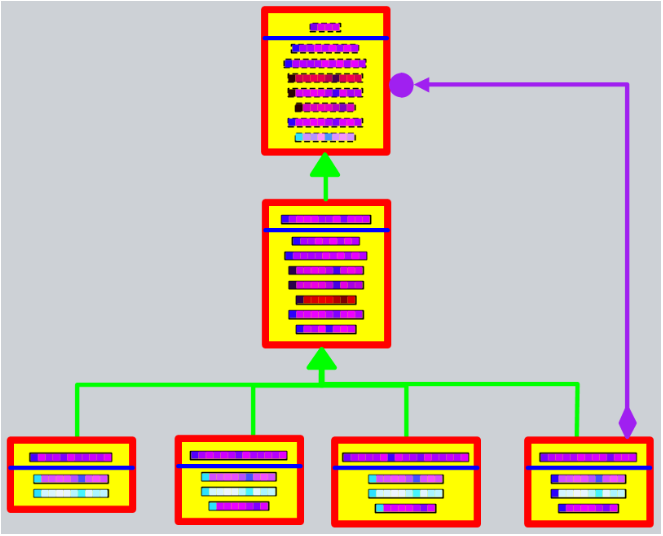
\includegraphics[scale=0.75]{figures/colored_uml.png}
    \caption{\textit{Colored UMl} für eine Mikroarchitektur}
    \label{fig:colored_uml}
\end{figure}

Die Abbildung \ref{fig:colored_uml} zeigt von Wang et al. erstelltes Exemplar für \textit{Colored UML}~\cite[S. 11]{app12178718}. Wie aus der Abbildung \ref{fig:colored_uml} zu entnehmen ist, werden Bezeichner, Modifizierer und Assoziationen farblich und/oder symbolisch encodiert.
Hierbei ist zu erwähnen, dass die Encodierung von Klassenattributen im Kontext dieser Arbeit von Wang et al, nicht berücksichtigt wird.
Die Rechtecke, die in Sektionen aufgeteilt sind, beschreiben die Klassen im Klassendiagramm. Die obere Sektion beinhaltet den Klassenbezeichner und dessen Modifizierer, während die untere Sektion die Methodennamen und deren Modifizierer beinhaltet. 
Jeder Bezeichner wird als Sequenz von Charakteren aufgefasst, in welchem für jeden Charakter algorithmisch eine Farbe aus dem Rot-Grün-Blau-Farbraum ermittelt wird~\cite[S. 9, S. 10]{app12178718}.
Modifizierer für Methoden werden als Teil der Charaktersequenz betrachtet und mitencodiert, während die Modifizierer für Klassen im Rand des Rechtecks encodiert werden, welches den Klassenbezeichner umschließt~\cite[S. 6]{app12178718}.
Die Kanten des Klassendiagramms, welche die Assoziationen zwischen Entitäten darstellen, werden in \textit{Colored UML} farblich annotiert und mit symbolisch an den Enden der Kanten je nach Art der Assoziation encodiert~\cite[S. 6]{app12178718}.

Zunächst werden im ersten Schritt des Prozesses aus Quelldateien durch Software-Werkzeuge UML-Klassendiagramme erstellt, welche im nächsten Schritt in \textit{Colored UML} umgewandelt werden.
Auf den encodierten Quelldaten wird der Bildklassifizierer VGGNet angewendet, welches Features aus der Eingabe als numerischen Vektor mit einer Länge von 1000 extrahiert. Im finalen Schritt dient dieser Feature-Vektor als Eingabe für eine Support Vector Machine, welches die Klassifikation übernimmt, zu welchem Entwurfsmuster die Eingabe zugeordnet werden kann~\cite[S. 13]{app12178718}.
Das hier präsentierte Modell wird für zwölf Design Patterns trainiert~\cite[S. 15]{app12178718}
Für das Training des Modells und die Evaluierung der Resultate des Verfahrens werden drei Open Source Software-Systeme verwendet. Zusätzlich wird das Verfahren mit drei nicht Machine Learning-Verfahren auf \textit{Precision} und \textit{Recall} verglichen~\cite[S. 20]{app12178718}.
Nach eigener Evaluierung von Wang et. al weist das ihrerseits entwickelte Verfahren verglichen zu den anderen Methoden ähnliche oder bessere Klassifizierungsleistung auf~\cite[S. 22]{app12178718}.

\pagebreak

Eine weitere Möglichkeit, um Entwurfsmuster im Quellcode zu ermitteln, ist die Extraktion von Metriken und Maßen aus dem Quellcode, die typisch für eine Instanz des betrachteten Design Pattern sind.
In ihrer Arbeit fokussieren sich Uchiyama et al. auf diesen Punkt und definieren einen Katalog aus Metriken und Maßen, der als Eingabe für einen Klassifizierer verwendet werden.
In dieser Arbeit definieren Uchiyama et al. Design Patterns als eine Summe von Strukturen, die im Kontext des Entwurfsmusters eine Rolle zugeordnet werden~\cite[S. 3]{Uchiyama2014}.
Dabei limitieren sich Uchiyama et al. auf die Erkennung von fünf Entwurfsmustern mit insgesamt 12 Rollen im Quellcode.~\cite[S. 4]{Uchiyama2014}.
Für diese Rollen werden Metriken und Maße ermittelt, die diese charakteristisch beschreiben.
Um die Elemente des Katalogs zu bestimmen, wird in dieser Arbeit die Goal-Question-Metric Methode angewendet~\cite[S. 4]{Uchiyama2014}.
Hierbei werden gezielt Fragen gestellt, mit dem Ziel, die jeweilige Rolle zu bestimmen. Für die Beantwortung dieser Fragen werden Metriken bzw. Maße definiert und als Teil des Katalogs aufgenommen.
Um die zwölf Rollen zu bestimmen, definieren Uchiyama et. al folgende Metriken~\cite[S. 7]{Uchiyama2014}:


\begin{table}[H]
    \centering
    \begin{tabular}{|c|c|}
        \hline
        Abkürzung & Beschreibung\\
        \hline
        NOF & Anzahl der Felder\\
        NSF & Anzahl der statischen Felder\\
        NOM & Anzahl der Methoden\\
        NSM & Anzahl der statischen Methoden\\
        NOI & Anzahl der implementierten Schnittstellen\\
        NOAM & Anzahl abstrakter Methoden\\
        NORM & Anzahl der überschriebenen Methoden\\
        NOPC & Anzahl der privaten Konstruktoren in der Klasse\\
        NOTC & Anzahl der Konstruktoren mit Objektparametern\\
        NOOF & Anzahl der an Feldern mit Objekttypen\\
        NCOF & Anzahl der anderer, die die Klasse/Schnittstelle als Feld referenzieren\\
        NMGI & Anzahl der Methoden, die Instanzen generieren\\
        \hline 
    \end{tabular}
    \caption{Metriken und Maße für Rollen nach Uchiyama et al.}
    \label{table:metrics}
\end{table}

Im ersten Schritt ihrer Methode extrahieren Uchiyama et al. die aus der Tabelle~\ref{table:metrics} definierten Metriken für jede Entität aus den Quelldateien. 
Diese Metriken werden als Vektor aufgefasst und diese werden als Eingabe für einen Klassifizierer verwendet, welche die Rollenzuweisung übernimmt~\cite[S. 5]{Uchiyama2014}.
Bei dem in dieser Methodik angewandten Klassifizierter handelt es sich um ein neuronales Netzwerk~\cite[S. 4]{Uchiyama2014}.
Die Ausgabe des Klassifizierers sind Werte, die angeben, mit welcher Sicherheit der Feature-Vektor zu der jeweiligen Rolle zugeordnet werden kann~\cite[S. 5]{Uchiyama2014}.
Anhand dieser Ausgabe werden die Rollen mit dem höchsten Konfidenzwert als Eingabe für die Bestimmung des Entwurfsmusters genommen. Unter der Berücksichtigung der Relationen der Rollen in dem Entwurfsmuster wird ein Übereinstimmungswert ermittelt, der angibt, mit welcher Wahrscheinlichkeit die Rollen zu dem jeweiligen Design Pattern passen.~\cite[S. 6]{Uchiyama2014}. Je höher dieser Wert, desto höher die Konfidenz, dass es sich hierbei um das Entwurfsmuster handelt.
Für das Training ihres Klassifizierers nutzen Uchiyama et al. 60 Instanzen aus klein-skalierten Software-Systemen und 158 aus drei größeren Open Source Software-Systemen.~\cite[S. 7]{Uchiyama2014}
Für die Evaluierung der Methode bedienen sich Uchiyama et. al den Metriken der \textit{Precision} und \textit{Recall} und ermitteln diese für ihr Verfahren.
Dabei werden für Instanzen aus klein-skalierten Software-Systemen bessere \textit{Precison}- und \textit{Recall}-Werte erzielt, verglichen zu den Werten für Instanzen aus den Open Source Software-Systemen~\cite[S. 8]{Uchiyama2014}

\smallbreak

Durch Charakterisierung der Klassen, Schnittstellen und Objekte durch Metriken und Maße sind zwar Rückschlüsse auf Struktur und Verhalten möglich, jedoch wird der lexigrafische und syntaktische Aspekt nicht mit berücksichtigt.
Um dagegenzuwirken, präsentieren Nazar et. al in ihrer Arbeit ihre Methode namens DPD\textsubscript{F}, die diese Aspekte des Quellcodes mitberücksichtigt~\cite[S. 1]{Nazar2020}.
Initial wird aus dem Quellcode durch statische Codeanalyse folgende Metriken extrahiert~\cite[S. 5]{Nazar2020}:

\begin{table}[H]
    \begin{tabular}{|c|c|}
        \hline
        Featurebezeichner & Beschreibung\\
        \hline
        ClassName & Name der Java Klasse\\
        ClassModifiers & Public, Protected und Private-Schlüsselwörter\\
        ClassImplements & Binäres Features (0/1), falls eine Schnittstelle implementiert wird\\ 
        ClassExtends & Binäres Features (0/1), ob Klasse von einer anderen vererbt\\
        MethodName & Methodenname in der Klasse\\
        MethodReturnType & Typ des Rückgabewerts einer Methode\\
        MethodBodyLineType & Art des Ausdrucks (z.B Variablenzuweisung, Boolean-Ausdruck)\\
        MethodNumVariables & Anzahl der Variablen/Attribute in der Klasse\\
        MethodNumMethods & Anzahl der Methodenaufrufe in der Klasse\\
        MethodsNumLine & Anzahl der Zeilen in Methode\\
        MethodIncomingMethod & Anzahl an Methoden, die in eine Methode aufruft\\
        MethodIncomingName & Name der Methoden, die von der Methode aufgerufen werden\\
        MethodOutgoingMethod & Anzahl ausgehender Methoden\\
        MethodOutgoingName & Name der ausgehenden Methoden\\
        \hline  
    \end{tabular}
    \caption{Extrahierte Features für DPD\textsubscript{F}}
    \label{table:dpdf_features}
\end{table}

Die ersten vier in der Tabelle \ref{table:dpdf_features} aufgelisteten Features werden pro Klasse ermittelt, während die restlichen elf für jede Methode in der Klasse bestimmt werden.
Jedes dieser Features wird als eine Auflistung von Schlüssel-Werte-Paaren in natürlicher Sprache formuliert.
Da die Ermittelung der Metriken für jede Methodendefinition durchgeführt wird, werden Features der Klasse in der Methodenevaluierung wiederholt.
Jede Evaluierung wird als Eintrag in einer Textdatei zusammengefasst. Das dabei entstehende Format wird von Nazar at al. als Syntactic and Lexical Representation (SSLR) benannt~\cite[S. 1]{Nazar2020}.
Um dieses Format in eine numerische Form zu bringen, wird SSLR als Eingabe für das Embedding-Modell Word2Vec verwendet, welches für jedes Token in der Eingabe durch Einbezug der umgebenden Tokens einen numerischen Vektor mit einer Länge von 100 determiniert, welches das jeweilige Token repräsentiert~\cite[S. 6]{Nazar2020}.
Die resultierenden Vektoren dienen als Eingabe für einen Random Forest Classifier, welches das meist passende Entwurfsmuster bestimmt~\cite[S. 7]{Nazar2020}.
Für das Training der Modelle und Evaluierung von DPD\textsubscript{F} wird ein eigener Korpus angelegt, bestehend aus Quelldateien aus \textit{Github Java Corpus}. Für die Evaluation und das Training werden zwölf Entwurfsmuster mit je 100 Instanzen aus dem Korpus genutzt, die durch Crowdsourcing identifiziert wurden~\cite[S. 4]{Nazar2020}.
Die Beurteilung der Resultate erfolgt durch die Bestimmung der \textit{f1}-, \textit{Precision}- und \textit{Recall}-Werte wird für jedes betrachtete Design Pattern. Nach eigener Evaluation erreicht ihre Methode mit dem selbsterstellten Datensatz im Durchschnitt einen \textit{Precision}-Wert von über 80\% und einen \textit{Recall}-Wert von 79\%~\cite[S. 8]{Nazar2020}.


\subsection{Query Ansätze}

Eine weitere Möglichkeit, um Design Patterns in Quellcode zu identifizieren, ist durch das Stellen von Anfragen an das Software-System.
Die Antwort auf die gestellte Anfrage ist dabei solch eine, die die in der Anfrage formulierten Bedingungen am besten befriedigt.
Solch einen Ansatz verfolgen Mäder et al. in ihrer Methodik. Dabei liegt der Fokus in ihrer Methode auf Annotationen im Quellcode,
die Aufschlüsse auf mögliche Entwurfsmuster geben. In ihrer Arbeit definieren Mäder et al. Annotation als Teil des Quellcodes, die keine direkte Einwirkung auf Programmsemantik haben~\cite[S. 521]{Ghula-2010} und bieten gleichzeitig zusätzliche Informationen für statische Analyse durch Software-Werkzeuge und für das Verständnis des Software-Systems an.
Initial wird ein Katalog von Annotationen definiert, welche manuell von Software-Entwicklern in Quellcode des Software-Systems aufgenommen wird~\cite[S. 521]{Ghula-2010}.

\begin{figure}[h]
    \centering
    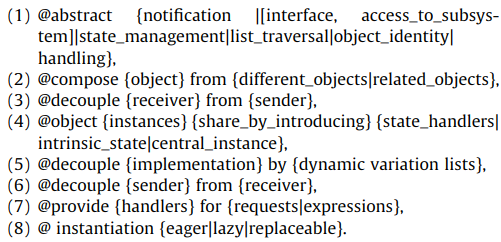
\includegraphics{figures/annotations.png}
    \caption{Ausschnitt an Annoation von Guhlam et al.}
    \label{fig:annotations}
\end{figure}

Abbildung \ref{fig:annotations} zeigt einen Ausschnitt des Annotationskatalogs, welcher im Kontext der Arbeit definiert wird. Dabei sind diese Annotationen so bestimmt, dass diese Informationen über die Struktur und Verhalten des Software-Artefakts widerspiegeln.
Der annotierte Quellcode wird im weiteren Verlauf durch das Software-Werkzeug Enterprise Architekt prozessiert. Dieses Werkzeug generiert ein Modell des Quellcodes und inkludiert die Beziehungen zwischen Software-Artefakten~\cite[S. 521]{Ghula-2010}. Informationen über Aggregation, Delegation und Freundschaften sind nicht Teil dieses Modells~\cite[S. 521]{Ghula-2010}.
Um die Existenz von Entwurfsmustern zu erkennen, wird ein Katalog an Regeln definiert, die verschiedene Aspekte von Design Patterns durch Mitberücksichtigung der Annotationen widerspiegelt~\cite[S. 523]{Ghula-2010}. Diese Regeln werden in SQL-Anfragen und reguläre Ausdrücke transformiert und in Sets von Regeln aufgeteilt, die auf die Existenz des zugewiesenen Design Patterns überprüfen~\cite[S. 523]{Ghula-2010}.  
Zu der Evaluierung ihrer Methode vergleichen Mäder et al. ihre Methode mit zwei anderen Verfahren. Dabei wird verglichen, welche Entwurfsmuster diese erkennen~\cite[S. 525]{Ghula-2010}.
Konkrete Metriken sind zu dem Zeitpunkt des Verfassens ihrer Arbeit nicht verfügbar~\cite[S. 525]{Ghula-2010}.

\pagebreak

Anstatt die Modellierung an ein professionelles Software-Werkzeug zu delegieren, entwerfen Stencel et al. ein eigenes Metamodell, wonach Entitäten aus dem Quellcode und ihre Relationen zueinander modelliert werden~\cite[S. 27]{stencel-2008}.
Dabei besteht das Metamodell aus Kernelementen wie types, attributes operations und instances und strukturellen und verhaltensbezogenen Relationen zwischen diesen Kernelementen. Sowohl die Kernelemente als auch die Relationen in diesem Metamodell sind möglichst ähnlich nach dem aus der objektorientierter Programmierung bekannten Verständnis definiert~\cite[S. 27]{stencel-2008}.
Jedes Design Pattern, das in dieser Arbeit betrachtet wird, wird von Stencel et al. in ihrem  Metamodell encodiert~\cite[S.28 - 29]{stencel-2008}. Diese dienen als Referenz für die Erkennung des jeweiligen Entwurfsmusters im Quellcode und werden als Grundlage für SQL-Anfragen genutzt~\cite[S. 29]{stencel-2008}.
In der Implementierung der Methode wird durch Strukturanalyse, Analyse des Datenflusses und Analyse der Methodenaufrufe Artefakte in das Metamodell transformiert und in einer relationalen Datenbank abgelegt.
Durch die SQL-Abfragen wird in der Datenbank nach Instanzen abgefragt, die die von der Referenzdefinition bereitgestellten Bedingungen erfüllen.
Zu Evaluierung vergleichen Stencel et al. ihre Methode mit zwei anderen und überprüfen anhand von Software-Systemen, welche Entwurfsmuster erkannt werden~\cite[S. 30]{stencel-2008}.
Als Resultat erkennt das hier erläuterte Verfahren mehr Instanzen an als die anderen Methoden~\cite[S. 29]{stencel-2008}.

\subsection{Diverse Ansätze}

%%TODO: Explain 2-4 other misc approaches; I AM SO FUCKING DONE
In ihrer Arbeit präsentieren Kramer et al. eine der frühesten Verfahren, um Entwurfsmuster in Quellcode zu erkennen.
Mit der Absicht, die Wartbarkeit von Software-Systemen zu verbessern, nutzen die Kramer et al. die Programmiersprache PROLOG, um 
Design Patterns als einzelne Regeln zu repräsentieren~\cite[S. 2]{Krammer-1996}. Diese dienen als Referenz im weiteren Verlauf der Methode.
Initial wird der zu verarbeitende Quellcode durch ein Software-Werkzeug in ein Object-Modelling Technique Diagramm transformiert und im nächsten Schritt wird das erstellte Diagramm in PROLOG-Code übersetzt.
Die als Referenz genutzten Definitionen der Entwurfsmuster dienen als Anfrage, die in dem transformierten Quellcode nach Instanzen des jeweiligen Design Patterns suchen~\cite[S. 2]{Krammer-1996}.
Zu Evaluierung werden von Kramer et al. die Definitionen für die Design Patterns Adapter, Bridge, Decorater und Proxy angelegt und die Methode an vier C++-Bibliotheken angewendet.
Nach eigener Evaluierung von Kramer et al. erzielt die Methode einen \textit{Precision}-Wert zwischen 14\% und 50\%~\cite[S. 7]{Krammer-1996}.

Anstatt ein Verfahren von Grund aus neu zu entwerfen, bedienen sich Binun et al. in ihrer Methode auf bereits etablierte Software-Werkzeuge und Methoden.
Sie erläutern, dass unterschiedliche Verfahren die einzelnen betrachteten Entwurfsmuster unterschiedlich präzise erkennen~\cite[S.15 - 17]{binun2009}.
In ihrer Methode wird die Ausgabe von fünf Verfahren zu einem finalen Wert zusammengefasst, der angibt, mit welcher Wahrscheinlichkeit es sich um das determinierte Design Pattern handelt.
Falls die einzelnen Methoden oder Werkzeuge die Eingabe unterschiedlich klassifizieren, wird versucht, durch die Identifikation einzelner Rollen im Quellcode das Entwurfsmuster zu rekonstruieren und dadurch die Eingabe einem Entwurfsmuster zuzuordnen~\cite[S. 15 - 16]{binun2009}.
Für die Evaluierung bedienen sie sich zwölf Software-Systeme als Eingabe für ihre Methode. In diesen wird nach Instanzen von fünf Entwurfsmustern gesucht~\cite[S. 9, S. 23]{binun2009}.
Nach eigener Evaluierung von Binun et al. werden drei von fünf Entwurfsmustern mit einem \textit{Precision}-Wert von über 70\% erkannt, während für die restlichen zwei mehrheitlich von den aggregierten Methoden nicht erkannt werden~\cite[S. 22]{binun2009}.



\chapter{Methodologie}
\section{Verfügbare Datensätze}\label{dataset}
Um ein Machine Learning Modell zu trainieren, benötigt es einen Datensatz mit passenden gekennzeichneten Klassen.
In der Erkennung von Entwurfsmustern existiert zu dem Zeitpunkt der Verfassung dieser Arbeit keine standardmäßiger oder weit akzeptierter Datensatz.
Jedoch existieren Versuche, solch einen Datensatz zu etablieren. Im Folgenden wird eine Auswahl an möglichen existierenden Datensätzen aufgelistet~\cite[S. 104 - 105]{phdthesis}:

\begin{description}
    \item Pattern-like Micro-Architecture Repository (P-MArt): Dieser Datensatz ist der einzige der hier aufgelisteten, welcher Peer-Reviews unterzogen wurde. Zwar bestehen die Autoren nicht darauf, dass alle möglichen Instanzen von Entwurfsmustern in den Software-Systemen identifiziert wurden, haben aber Zuversicht, dass die Mehrheit der Instanzen durch mehrfache Analysen durch mehrere Teams erkannt wurde. 
    \item DEsign pattern Evaluation BEnchmark Environment (DEEBEE): Dieser Datensatz beinhaltet Resultate aus automatischer und einer manuellen Analyse von fünf Software-Systemen auf Entwurfsmustern.
    \item Design Pattern Benchmark (DPD): DPD beinhaltet die Ergebnisse von Software-Systemen durch mehrere Software-Werkzeuge. Zudem sind die Daten des Datensatzes durch eine Webseite verfügbar, in der nach Instanzen von Entwurfsmustern in Software-Systemen gesucht werden kann. Zusätzlich können auf dieser Webseite Ergebnisse evaluiert und durch öffentlich zugängliche Abstimmung einer Instanz das passende Design Pattern zugeordnet werden.
    \item PattErn Repository and Components Extracted from OpeN Source software (PERCERONS): PERCERONS ist das derzeit von dem Umfang her der größte verfügbare Datensatz mit über 537 analysierten Software-Systemen. Die Ergebnisse wurden durch das Kombinieren der Resultate zweier Software-ErgebnisWerkezeuge ermittelt.
    \item Software Engineering Research Center benchmark (SERC): SERC wurde konstruiert, um als Vergleichsmaßstab für ein Software-Werkzeug zu dienen, welches von den gleichen Autoren stammte. Dabei werden die Ergebnisse von mehreren anderen Werkzeugen mit den Ergebnissen ihres eigenes kombiniert.
\end{description}

Die Problematik bei der Ermittelung eines geeigneten Datensatzes besteht darin, dass der Umfang der analysierten Software-Systeme sich in Grenzen hält und meist eher als Maßstab für die Leistung der selbst entwickelten Methode verwendet wird, wodurch Bias zu der eignen Methode nicht ausgeschlossen werden kann.
Zudem sind die hier aufgeführten Datensätze bis auf einige Ausnahmen durch die Kombination von mehreren Software-Werkzeugen entstanden. Durch solch ein Verfahren ist zwar die Analyse von mehreren Software-Systemen in einer relativ kurzen Zeitspanne möglich, jedoch wäre eine manuelle Verifizierung der Ergebnisse aufgrund von hohen Zeit- und Leistungsaufwands schwer umsetzbar.
Dahingegen wäre das ideale Vorgehen, das solch ein Datensatz durch manuelles Identifizieren von Entwurfsmustern in Quellcode durch die Analyse von mehreren Software-Systemen durch ein Experten-Team erstellt wird. Jedoch ist solch ein Verfahren zeitaufwendig und erfordert ein tiefes Verständnis des jeweiligen Software-Systems, welches durch mangelnde oder obsolete Dokumentation eine Hürde darstellt.
Die nächst bestmögliche Alternative dazu ist die Option des Crowdsourcings wie in DPD. Das Problem ist hier, dass die Qualifikation der Personen, die Instanzen von Entwurfsmustern identifizieren und über die korrekte Zuweisung abstimmen, nicht garantiert sind. Zudem erfordert dies ein Publikum mit der Bereitschaft, dies zu tun, welches auch nicht garantiert werden kann.
Bei dem im Kontext dieser Arbeit vorgestellten Verfahren für die Ermittelung von Entwurfsmustern wird meist ein Datensatz im kleinen Umfang erstellt. Auf Anfrage. um Zugang zu einigen Datensätzen zu erhalten, gibt es zu dem Zeitpunkt zur Verfassung dieser Arbeit keine Antwort seitens der Autoren. Zudem sind die Webseiten, worüber auf die Datensätze zugegriffen werden kann, nicht mehr verfügbar und der Zugang über eine Archivierungsdienstleistung wie der Wayback Maschine war ebenfalls nicht möglich. 
Aus den hier aufgelisteten Gründen wird im Zuge dieser Arbeit der P-MArt Datensatz verwendet und somit die Untersuchungsfrage~\ref{RQ2} zu beantworten. Dieser ist zum Zeitpunkt des Verfassens dieser Arbeit zugänglich und ist der Einzige, der Peer-Reviews unterzogen wurde. In der Sektion der Implementierung wird dieser genauer betrachtet.
\section{Feature Engineering}
\section{Modellauswahl, Training und Validierung}
Nach dem Bestimmen eines passenden Datensatzes und zu extrahierenden Features wird ein Klassifizierer trainiert, welcher mit einem Wahrscheinlichkeitswert angibt, welche Rolle am ehesten der Quellcodeentität zugeordnet werden kann.
Dazu wird in dieser Sektion erläutert, welche Modelle betrachtet werden und wie diese trainiert und evaluiert werden können. 


\subsection*{Auswahl der Klassifizierer}
Im Zuge dieser Arbeit werden in der Sektion \ref{classifiers} erläuterten Klassifizierer als die bevorzugten Modelle hergenommen. Diese Auswahl der Modelle ist auf unterschiedliche Gründe zurückzuführen.
Klassifizierer können je nach Art und Weise, wie sie innerlich funktionieren, in Kategorien untergliedert werden. Dabei dienen die Modelle aus Sektion \ref{classifiers} als Repräsentanten ihrer Kategorie, sodass ein Spektrum von unterschiedlich funktionierenden Modellen getestet werden kann.
Ohne das Testen des jeweiligen Models ist dessen Leistung für das in dieser Arbeit genutzten Datensatzes nicht vorherzusagen. Zudem können Implementierungen der jeweiligen Modelle in verschiedenen Programmiersprachen für verschiedene Plattformen vorgefunden werden.
Dies ermöglicht die Nutzung in Programmiersprachen wie Python oder R, welche für Machine Learning bevorzugt werden. Das Software-Framework, welches die Implementierungen für die Modelle zur Verfügung stellt und im Kontext dieser Arbeit angewendez wird, wird im weiteren Verlauf der Arbeit genauer erläutert.
Der größte Vorteil dieser Klassifizierer ist deren Simplizität und damit resultierende Effizienz in Zeit- und Speicherkomplexität. Da die Klassifizierer im weiteren Verlauf der Methode durch den Einsatz von Hyperparameter-Tuning iterativ optimiert werden, ist dies von besonderer Bedeutung.
Deshalb werden Modelle mit komplexerer Architektur aufgrund des Mangels verfügbarer Rechenressourcen zu Zeitpunkt des Verfassens der Arbeit nicht weiter betrachtet. 
Die Auswahl der Klassifizierer aus Sektion~\ref{classifiers} beantwortet die Untersuchungsfrage~\ref{RQ5}


\subsection*{Training der Modelle}
In dieser Arbeit wird das Trainieren der Modelle mit dem Hyperparameter-Tuning aus Sektion~\ref{hyper_params} gekoppelt. Zuerst wird der Datensatz in ein Trainings- und Validationsdatensatz aufgeteilt. Danach wird für jedes Modell ein Suchraum für die Hyperparameter-Werte, Anzahl der Trainingsiterationen und die Metrik bestimmt, wonach die Leistung des Klassifizierers
beurteilt wird. In jeder Iteration wird zufällig eines der hier vorgestellten Klassifizierer mit einer vorher bestimmten Hyperparameter-Konfiguration instanziiert, mit dem Trainingsdatensatz trainiert und durch Einsatz des Validationsdatensatzes der Wert der Leistungsmetrik bestimmt. Die Hyperparameter-Konfiguration der Instanz mit der besten Leistung aus allen Iterationen wird im weiteren Verlauf der Arbeit verwendet.

\subsection*{Validierung des Modells}
Dadruch, dass der Datensatz für das Training aufgeteilt wird, wird die beste Hyperparameter-Konfiguration eines der hier vorgestellten Klassifizierer durch Kreuzvalidierung zusätzlich validiert. 
Dabei wird der gesamte verfügbare Validationsdatensatz verwendet. Die Evaluierung der Leistung der Klassifikationskapazität erfolgt mit der gleichen Metrik wie in der Trainingsphase. Es bestünde die Option, dass man die Kreuzvalidierung direkt in die Trainingsphase integriert. 
Jedoch ist dabei zu beachten, dass die Kreuzvalidierung selbst iterativ agiert und dies in jeder Iteration des Hyperparameter-Tunings durchgeführt wird. Dies erhöht die Laufzeit der Trainingsphase signifikant.
\section{Evaluation des trainierten Models}
\section{Ermittelung übereinstimmendes Design Patterns}

\chapter{Implementierung}
\section{Präprozessierung des Datensatzes}\label{data_preprocessing}
Wie in Sektion~\ref{dataset} erläutert, wird in dieser Arbeit der Datensatz P-MArt verwendet.
P-MArt ist ein Katalog von Design Pattern mit Instanzen aus mehreren Software-Systemen. 
Dabei wird bei jeder Instanz eines Design Pattern die aufkommenden Software-Entitäten wie Klassen oder Schnittstellen mit Rollen nach Gamma et al. annotiert.

\begin{table}[H]
    \centering
    \begin{tabular}{|p{0.2\linewidth}|p{0.55\linewidth}|p{0,25\linewidth}|}
        \hline
        Projekt & Beschreibung & Programmiersprache\\
        \hline
        QuickUML 2001 & An Anfänger gerichtetes Werkzeug für die Erstellung UML-Diagrammen & Java\\
        Lexi v0.1.1 alpha & einfaches Textverarbeitungssystem & Java\\
        JRefactory v2.6.24 & Software-Werkzeug für das Refactoring für Java & Java\\
        Netbeans v1.0.x & integrierte Entwicklungsumgebung für Software & Java\\
        JUnit v3.7 & Test-Framework für Java-Projekte & Java\\
        JHotDraw v5.1 & Framework für das Erstellen von Editoren & Java\\
        MapperXML v1.9.7 & Presentation-Framework & Java\\
        Nutch v0.4 & Open Source Suchmaschine für das Web & Java\\
        PMD v1.8 & Werkzeug für statische Codeanalyse & Java\\
        Software architecture design patterns in Java & Kollektion von Implementierung von Design Patterns nach Kuchana~\cite{10.5555/983553} & Java\\
        DrJava v20020619 & integrierte Entwicklungsumgebung für Java & Java\\
        DrJava v20020703 & integrierte Entwicklungsumgebung für Java & Java\\
        DrJava v20020804 & integrierte Entwicklungsumgebung für Java & Java\\
        DrJava v20030203 & integrierte Entwicklungsumgebung für Java & Java\\
        \hline
    \end{tabular}
    \caption{Software-Systeme in P-MArt}
    \label{tab:pmart_projects}
\end{table}

Tabelle~\ref{tab:pmart_projects} listet die Software-Systeme auf, die in P-MArt betrachtet werden. Dabei sind alle Software-Systeme in der Programmiersprache Java verfasst und unterliegen einer Open-Source-Lizenz, wodurch der Quellcode frei zugänglich ist.
Zudem waren nicht alle Software-Systeme zugänglich. Die verschiedenen Versionen der Entwicklungsumgebung DrJava waren archiviert über die Webplattform SourceForge verfügbar. Das Werk "Software architecture design patterns in Java" von Kuchana ist ein Fachbuch für den Einsatz von Design Pattern in Java. 
In P-MArt werden die Software-Beispiele inkludiert, die im Kontext des Werkes zur Erläuterung dienen und durch die Webplattform des Verlags zugänglich ist. Die im Werk erwähnte URL für die Bespiele zu dem Zeitpunkt der Verfassung der Arbeit nicht zugänglich.
Der Quellcode für die restlichen Software-Systeme ist als Archiv über die Webseite der Autoren zugänglich.

P-MArt selbst wird in der Form einer Extensible Markup Language (XML) Datei verfügbar gestellt. Für einfachere Verarbeitung des Datensatzes werden die notwendige Information aus der XML-Datei extrahiert und in einer Comma-Separated Values (CSV) Datei abgelegt.

\begin{table}[H]
    \centering
    \begin{tabular}{|c|c|}
        \hline
        Spalte & Beschreibung\\
        \hline
        project & Name des Software-Systems\\
        micro\_architecture & Identifikator der Mikroarchitektur in P-MArt\\
        design\_pattern & Zugeordnetes Entwurfsmuster nach Gamma et al.\\
        role & Rolle der Entität innerhalb des Design Patterns nach Gamma et al.\\
        role\_kind & Art der Entität (\textit{Class} für Klasse oder \textit{AbstractClass} für abstrakte Klassen)\\
        entity & qualifizierender Name der Entität innerhalb des Software-Systems\\
        \hline
    \end{tabular}
    \caption{Spalten der prozessierten CSV-Datei für P-MArt}
    \label{tab:pmart_roles}
\end{table}

Die Tabelle~\ref{tab:pmart_roles} zeigt die Spalten der resultierenden CSV-Datei. Für die Erstellung dieser Datei wird die Skriptsprache Python und dessen Standardbibliothek verwendet.
Neben den in Tabelle~\ref{tab:pmart_roles} aufgeführten Informationen beinhaltet die beschreibende XML-Datei von P-MArt zusätzliche Details wie Kommentare der Autoren über einzelne Mikroarchitekturen.
Diese werden in der weiteren Verarbeitung der Daten nicht berücksichtigt. Die resultierende CSV-Datei dient zusammen den Quellcode der in P-MArt analysierten Software-Systeme als Eingabe für die Extraktion der Features.

\section{Extraktion von Features aus Quellcode}
\section{Analyse des Datensatzes}\label{dataset_analysis}

In der Sektion~\ref{feature_extraction} wird der Datensatz verarbeitet und mit den in Tabelle~\ref{tab:features} erweitert.
In diesem Abschnitt wird das Resultat der Sektion~\ref{feature_extraction} analysiert.
Für den weiteren Verlauf der hier vorgestellten Methode wird die Skriptsprache Python in Kombination mit Jupyter-Notebooks benutzt. Für die Analyse der Daten wird Python-Bibliothek pandas verwendet. Für die Visualisierung durch verschiedene Arten von Diagrammen wird die Python-Bibliothek plotly eingesetzt.


\begin{table}[h]
    \begin{tabular}{|c|c|}
        \hline
        Entwurfsmuster & Anzahl\\
        \hline
        Singleton&15\\Adapter&9\\Command&8\\Observer&6\\Strategy&6\\Iterator&6\\Factory Method&5\\Template Method&5\\Composite&5\\Proxy&4\\Memento&4\\Builder&4\\Visitor&4\\State&3\\Abstract Factory&3\\Decorator&2\\Facade&1\\Bridge&1\\Null Object&1\\Prototype&1\\FactoryMethod&1\\Mediator&1\\
        \hline
    \end{tabular}
    \caption{Verteilung der Entwurfsmuster in P-MArt}
    \label{tab:dp_dist}
\end{table}



Die Tabelle~\ref{tab:dp_dist} zeigt die Verteilung der Instanzen der Design Pattern an. 
Dabei ist abzulesen, dass die Singelton-, Adapter-, Command- und Observer-Entwurfsmuster die am häufigsten vertretenen Entwurfsmuster sind, während Instanzen der Design Patterns wie Decorator oder Bridge nur einmal vorkommen.
Dies beantwortet die Untersuchungsfrage~\ref{RQ1}.

\pagebreak

\begin{figure}[h]
    \centering
    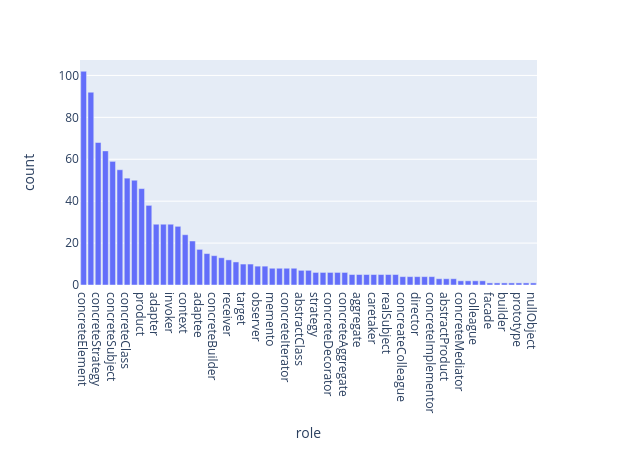
\includegraphics[scale=0.6]{figures/role_dist.png}
    \caption{Rollenverteilung in P-MArt}
    \label{fig:role_dist}
\end{figure}

Abbildung~\ref{fig:role_dist} ermöglicht einen Überblick über die Rollenverteilung.
Dabei ist zu vermerken, dass die Verteilung der Rollen und die Anzahl der Instanzen der zugehörigen Design Pattern unbalanciert ist. Beispielsweise ist die Rolle \textit{concreteelement} des Visitor-Entwurfsmusters am häufigsten vorzufinden, obwohl in P-MArt vier Instanzen vermerkt sind.
Um ein möglichst aussagekräftiges Ergebnis zu erhalten, muss die Menge der zu identifizierenden Entwurfsmuster eingeschränkt werden. Ansonsten ist bei zu vielen identifizierbaren Klassen mit wenigen Datenpunkten eine unzufriedenstellende Leistung der Klassifizierer zu erwarten.
Deshalb werden im weiteren Verlauf Instanzen der Entwurfsmuster Singelton, Observer, Command und Adapter weiter betrachtet.


\begin{table}[H]
    \begin{tabular}{|c|c|c|}
        \hline
        Entwurfsmuster & Rolle & Anzahl\\
        \hline
        Singelton & singelton & 15\\
        \hline
        \multirow{4}{*}{Adapter} & adaptee & 17\\ & adapter & 29\\ & client & 13\\ & target & 10\\
        \hline
        \multirow{5}{*}{Command} & client & 13\\ & command & 6\\ & concreteCommand & 50\\ & invoker & 29\\ & receiver & 12\\
        \hline
        \multirow{4}{*}{Observer} & concreteObserver & 28\\ & concreteSubject & 59\\ & observer & 9\\ & subject & 5\\
        \hhline{|=|=|=|}
        Insgesamt & & 295\\
        \hline
    \end{tabular}
    \caption{Aufteilung des Datensatzes für Training und Validierung}
    \label{tab:dataset_dist}
\end{table}

Tabelle~\ref{tab:dataset_dist} zeigt den Datensatz an, der im weiteren Verlauf verwendetet wird. Auf vier Design Pattern aufgeteilt,
beträgt der Umfang des Datensatzes 295 Datenpunkte auf vierzehn Rollen aufgeteilt.

\begin{figure}[h]
    \centering
    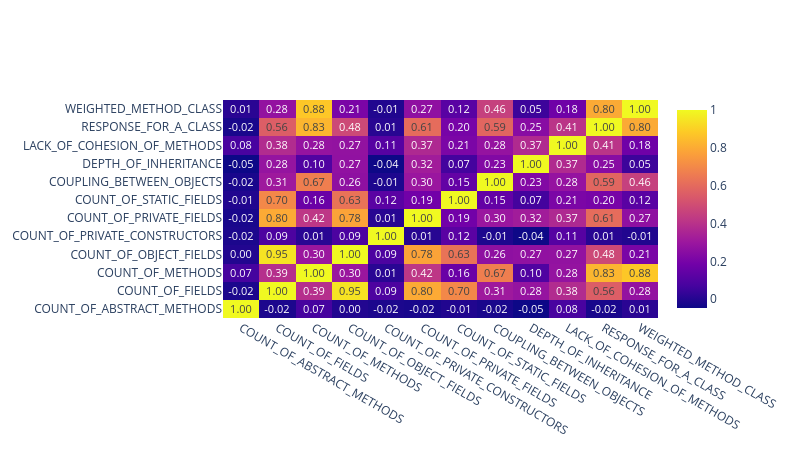
\includegraphics[scale=0.5]{figures/coff_heat_map.png}
    \caption{Koeffizienten-Heatmap der Features}
    \label{fig:coeff_heat_map}
\end{figure}

\pagebreak

Abbildung~\ref{fig:coeff_heat_map} beschreibt die Koeffizienten der Korrelation der einzelnen Features zueinander. Der Koeffizient der Korrelation wird paarweise für jede Metrik ermittelt.
Dabei kann der Koeffizient wie gefolgt interpretiert werden:

\begin{itemize}
    \item Zwischen -1.0 und 0: Dies wird als eine negative Korrelation bezeichnet. Je größer der eine Wert, desto kleiner wird der andere. Je kleiner der Koeffizient, desto größer der Einfluss.
    \item Gleich 0: Keine Korrelation ist vorzufinden.
    \item Zwischen 0 und 1.0: Ein Koeffizient in diesem Wertebereich wird als positive Korrelation benannt. Je größer der eine Wert, desto größer wird der andere. Je größer der Koeffizient, desto größer der Einfluss.
\end{itemize}

Bei der Datenanalyse von Features kann eine Koeffizienten-Heatmap dazu verwendet, um gegebenenfalls Features aus dem Featurevektor, um dessen Dimensionalität zu reduzieren. Die Dimensionalität beschreibt in diesem Kontext Anzahl der Komponenten im Featurevektor.
Je höher die Dimensionalität, desto mehr Möglichkeiten müssen berücksichtigt werden, um im Falle der Klassifikation eine möglichst passende Klasse zuzuordnen. Je kleiner die Dimensionalität, desto präziser kann klassifiziert werden.
Features mit einer besonders geringen oder hohen Koeffizient der Korrelation zu einer anderen encodieren ähnliche oder gleiche Informationen über die Entität, weshalb diese unter Umständen nicht mehr als Eingabe für Klassifizierer berücksichtigt werden.
Im Falle der Heatmap aus Abbildung~\ref{fig:coeff_heat_map} sind besonders hohe Koeffizienten der Korrelation vorzufinden. Jedoch werden unter Berücksichtigung des Domainwissens die alle Features für die Klassifikation verwendet
  




\section{Training und Validation der Klassifizierer}

Die in Sektion~\ref{classifiers} beschriebenen Klassifizierer, Random Forest Classifier, Support Vector Machine (SVM) und k-Nearest-Classifier (KNN) werden verwendet.
Die Implementierung dieser Klassifizierer und andere Funktionalitäten werden durch die Machine Learning Bibliothek scikit-learn~\cite{scikit-learn} zur Verfügung gestellt.
Der Prozess der Optimierung und das Training der Klassifizierer wird durch die Bibliothek hyperopt-sklearn~\cite{Komer2019} realisiert. 
Dabei kann der Trainingsprozess in folgende Schritte unterteilt werden:

\begin{enumerate}
    \item \textbf{Aufteilen des Datensatzes}: Für das Training wird der Datensatz aus Sektion~\ref{dataset_analysis} in einen Trainings- und Validationsdatensatz aufgeteilt. Dabei werden 70 \% der Datenpunkte dem Trainingsdatensatz und die restlichen 30 \% dem Validationsdatensatz zugewiesen. Die Rollen, die als Python String dargestellt werden, werden durch einen sklearn LabelEncoder ein kategorischer Integer-Wert zugewiesen. 
    \item \textbf{Initialisierung der Klassifizierer}: Die Instanzen der Klassifizierer werden mit den Standardwerten für die Hyperparameter initialisiert, die von hyperopt-sklearn zur Verfügung gestellt werden.
    Zusätzlich wird für jedes Modell einen Zahlenwert zwischen 0.0 und 1.0 definiert. Dieses gibt an, mit welcher Wahrscheinlichkeit das jeweilige Modell in einer Trainingsiteration ausgewählt wird. Falls notwendig, wird bei der Instanziierung der Klassifizierer ein zusätzlicher Schritt für die Skalierung der Werte der Datenpunkte durchgeführt.
    Dies ist der Fall bei SVM oder KNN, da bei unskalierten Datenwerten die Klassifikationsleistung von SVM und KNN negativ beeinträchtigt werden kann. Dabei wird der durch sklearn zur Verfügung gestellte StandardScaler verwendet, der Features standardisiert, indem dieser den Mittelwert entfernt und die Datenpunkte auf Einheitsvarianz skaliert. Für den Random Forrest Classifier wird die Skalierung der Datenpunkte ebenfalls angewandt, obwohl dessen Leistung davon nicht negativ beeinträchtigt wird.
    \item \textbf{Starten des Trainings}: Wie bereits erwähnt, wird das Training und Optimieren der Modelle durch hyperopt-sklearn automatisiert durchgeführt. Die Instanzen der Klassifizierer werden in einer Instanz der Klasse HyperoptEstimator gebündelt, welche als Abstraktionsschicht das Training und das Optimieren der Hyperparameter kapselt. Bei dessen Instanziierung wird ebenfalls bestimmt, wie viele Iterationen die Modelle für das Training insgesamt durchlaufen müssen, nach welcher Metrik die Iterationen evaluiert und nach welchem Algorithmus die Permutationen der Hyperparameter-Werte bestimmt werden. 
    Für das Training werden 20 Iterationen hergenommen und die Evaluation jeder Iteration erfolgt durch Ermittelung des \textit{f1}-Wertes. Für die Ermittelung der nächsten Konfiguration an Hyperparameter-Werten wird Tree of Parzen Estimators verwendet.
    \item \textbf{Kreuzvalidierung der besten Iteration}: Mit einem k-Wert von 5 wird die Kreuzvalidierung mit dem Validationsdatensatz und dem \textit{f1}-Wert als Evaluierungsmetrik an dem optimierten Model durchgeführt.
\end{enumerate}
\section{Bestimmung des Design Patterns}

\begin{algorithm}
    \caption{Funktion zur Bewertung von Rollenübereinstimmungen}
    \label{pattern_matching}
    \begin{algorithmic}[1]
    \Require $role\_encoder$: Der LabelEncoder für Rollen; 
    \Require $roles\_df$: Pandas DataFrame mit Rollendaten
    \Require $model$: Trainiertes Modell zur Vorhersage von Rollen
    \Require $dps$: Hash Map mit Rollendefinitionen pro Entwurfsmuster
    
    \Function{match\_pattern}{$role\_encoder$, $roles\_df$, $model$, $dps$}
    
        \State $X \gets$ \Call{get\_feature\_columns}{$roles\_df$}
        \State $y \gets model.predict(X)$
        \State $roles \gets role\_encoder.inverse\_transform(y.ravel())$
        \State $scores \gets$ leere Hash Map
        \State $predicted\_role\_freq \gets$ leere Hash Map
        
        \ForAll{$role$ in $roles$}
            \State $predicted\_role\_freq[role] \gets predicted\_role\_freq[role] + 1$
        \EndFor
        
        \ForAll{$dp, dp\_roles$ in $dps$}
            \State $matched\_roles \gets$ leere Hash Map
            \State $dp\_roles\_dict \gets$ Konvertiere $dp\_roles$ zu Hash Map
            
            \ForAll{$role$ in $predicted\_role\_freq$}
                \If{$role$ in $dp\_roles\_dict$}
                    \State $dp\_role \gets dp\_roles\_dict[role]$
                    \If{($dp\_role.mutliple\_occurences$ oder $predicted\_role\_freq[role] = 1$) und $matched\_roles[role] < predicted\_role\_freq[role]$}
                        \State $matched\_roles[role] \gets matched\_roles[role] + 1$
                    \EndIf
                \EndIf
            \EndFor
            
            \State $total\_possible\_matches \gets$ Summe der möglichen Übereinstimmungen
            \State $score \gets$ Berechne Übereinstimmungswert
            \State $scores[dp] \gets score$
        \EndFor
        
        \State \Return $scores$
    \EndFunction
    \end{algorithmic}
\end{algorithm}
    
Der Pseudocode~\ref{pattern_matching} beschreibt die konkrete Implementierung des in der Sektion~\ref{pattern} erläuterten Algorithmus.
Dabei wird trainierte Klassifizierer initialisiert, die Metriken aus~\ref{tab:features} für die zu klassifizierenden Entitäten aus der Quellcode ermittelt und als Eingabeparameter für die vorgestellte Funktion verwendet.
Die Berechnung des Übereinstimmungswertes erfolgt, indem zunächst die Gesamtzahl möglicher Übereinstimmungen bestimmt wird, die sowohl einmalige als auch mehrfache Vorkommen von Rollen berücksichtigt. Der Übereinstimmungswert für jedes Entwurfsmuster wird als das Verhältnis der Anzahl abgeglichener Rollen zur Gesamtzahl möglicher Übereinstimmungen berechnet. 
Dieser Wert gibt an, wie gut die vorhergesagten Rollen mit den für das Design Pattern definierten Rollen übereinstimmen. Der höchste Übereinstimmungswert wird als bestmögliche Antwort betrachtet.
\section{Evaluation der Ergebnisse}

\chapter{Schluss}
\section{Fazit}

Zusammenfassend ist das Ergebnis dieser Arbeit als negativ zu beurteilen. Zwar ist der Algorithmus für das Zuweisen der Entwurfsmuster in der Lage, teilweise das korrekte Design Pattern zuzuordnen,
jedoch ist dessen Aussagekraft von der Leistung des Klassifizierer abhängig. Wie in der Sektion der Evaluation erläutert, ist als mangelhaft zu beurteilen.
Die Problematik besteht darin, dass es für das Trainieren von Maschine-Learning-Modellen für Klassifikationsaufgaben keine definitiven Prozesse existieren.
Dies gilt vor allem für die Bestimmung der Features, welches durch den verfügbaren Datensatz und dessen Qualität und Umfang limitiert ist. 
Wie in Sektion~\ref{dataset_analysis} zu sehen ist, ist das Verhältnis zwischen Datenpunkten und Design Pattern von dem Umfang der einzelnen Implementierungen abhängig. Dadurch, dass die Design Patterns so unbalanciert im Datensatz repräsentiert, kann es vorkommen,
dass einige Design-Pattern-Rollen überrepräsentiert, während andere unterrepräsentiert sind. Zudem ist Konfiguration der Hyperparameter ebenfalls eine weitere Methode,
um die Klassifikationsleistung zu verbessern. Zwar stellen automatisiertes Hyperparameter-Tuning und der Einsatz von Kreuzvalidierung eine Option dar, um die Leistung des Klassifizierers zu optimieren und zu validieren,
jedoch ist das beste Ergebnis dadurch nicht garantiert. Es besteht immer Wahrscheinlichkeit, dass die bestmögliche Konfiguration an Hyperparameter-Werten außerhalb des Suchraumes liegt.

Insgesamt gesehen ist es davon auszugehen, dass verschiedene Aspekte und Optionen existieren, um den hier vorgeschlagene Methode weiter zu verbessern. 
Entweder kann beispielsweise ein anderer Katalog an Metriken als Features genutzt werden oder es werden andere Klassifizierer verwednet.


\section{Zukünftige Aussichten}

Die fortschrittlichen Entwicklungen im Bereich des maschinellen Lernens (ML) und speziell der Large Language Models (LLMs) eröffnen neue Perspektiven für die automatisierte Erkennung von Design Patterns in Quellcode. In dieses Feld wurden zum Zeitpunkt der Verfassen der Arbeit Fortschritte getätigt, da LLMs das Potenzial geben, die Effizienz und Genauigkeit bei der Identifizierung von Design Patterns erheblich zu verbessern. Im Folgenden werden die zukünftigen Aussichten dieser Technologie beleuchtet.

\begin{enumerate}
    \item \textbf{Erweiterte Erkennungskapazitäten}: Mit der zunehmenden Verfeinerung von LLMs ist zu erwarten, dass ihre Fähigkeit, komplexe Muster und Abstraktionen im Quellcode zu erkennen, deutlich zunimmt. Diese Modelle können aus einer umfangreichen Datenmenge lernen und somit eine breite Palette von Design Patterns identifizieren, die in verschiedenen Programmiersprachen und -stilen zum Einsatz kommen. Die Flexibilität von LLMs ermöglicht es ihnen, auch seltene oder weniger dokumentierte Patterns zu erkennen, die herkömmliche Methoden möglicherweise übersehen.
    \item \textbf{Verbesserung der Präzision und Reduzierung von Fehlalarmen}: Durch das Training mit großen Datensätzen können LLMs nicht nur eine Vielzahl von Patterns erkennen, sondern auch den Kontext, in dem diese Patterns verwendet werden, besser verstehen. Dies führt zu einer höheren Präzision bei der Erkennung und einer signifikanten Reduzierung von Fehlalarmen. Die Fähigkeit, den Kontext zu berücksichtigen, ist besonders wichtig, da viele Design Patterns nur in bestimmten Situationen angemessen sind. LLMs können feine Unterschiede im Code erfassen, die darauf hinweisen, ob ein bestimmtes Pattern tatsächlich beabsichtigt ist oder nicht.
    \item \textbf{Automatisierte Verbesserungsvorschläge und Refactoring}: Zukünftige Entwicklungen könnten LLMs befähigen, nicht nur existierende Patterns zu erkennen, sondern auch Verbesserungsvorschläge zu machen. Basierend auf der erkannten Implementierung eines Design Patterns könnten diese Modelle Empfehlungen für ein effizienteres oder klareres Pattern geben, das in den aktuellen Code eingeführt werden kann. Darüber hinaus ist das Potenzial für automatisiertes Refactoring beträchtlich, wobei LLMs Vorschläge für Code-Umstrukturierungen machen können, um Design Principles wie SOLID besser einzuhalten.
    \item \textbf{Interaktive Entwicklungsumgebungen}: Die Integration von LLMs in Entwicklungsumgebungen und IDEs (Integrated Development Environments) könnte zu einer interaktiveren und unterstützenden Codierungserfahrung führen. Entwickler könnten in Echtzeit Feedback zu den von ihnen verwendeten Design Patterns erhalten, einschließlich Hinweisen zur Anwendung und möglichen Optimierungen. Diese Art der direkten Integration fördert ein tieferes Verständnis für Design Patterns und unterstützt Entwickler dabei, best practices effektiver in ihren Code zu integrieren.
\end{enumerate}




\appendix
\chapter{Zusätzliche Tabellen für die Datenanalyse von P-MArt}


\begin{table}[H]
    \centering
    \begin{tabular}{|c|c|}
        \hline
        Rolle & Aufkommen in Datensatz\\
        \hline
        abstractclass & 7\\abstractfactory & 2\\abstraction & 1\\abstractproduct & 3\\adaptee & 17\\adapter & 29\\aggregate & 5\\builder & 1\\caretaker & 5\\client & 64\\colleague & 2\\command & 6\\component & 7\\composite & 11\\concreatecolleague & 4\\concreteaggregate & 6\\concretebuilder & 14\\concreteclass & 51\\concretecommand & 50\\concretecomponent & 55\\concretecreator & 13\\concretedecorator & 6\\concreteelement & 102\\concretefactory & 8\\concreteimplementor & 4\\concreteiterator & 8\\concretemediator & 2\\concreteobserver & 28\\concreteproduct & 38\\concreteprototype & 3\\concretestate & 21\\concretestrategy & 68\\concretesubject & 59\\concretevisitor & 29\\context & 24\\creator & 6\\decorator & 1\\director & 4\\element & 5\\facade & 1\\implementor & 1\\invoker & 29\\iterator & 4\\leaf & 92\\mediator & 2\\memento & 8\\nullobject & 1\\objectstructure & 4\\observer & 9\\originator & 8\\product & 46\\prototype & 1\\proxy & 5\\realsubject & 5\\receiver & 12\\refinedabstraction & 3\\singleton & 15\\state & 5\\strategy & 6\\subject & 9\\subsystemclass & 10\\target & 10\\visitor & 5\\
        \hline
    \end{tabular}
    \caption{tabellarische Darstellung der Rollenverteilung in P-MArt}
\end{table}

%%% Local Variables: 
%%% mode: latex
%%% TeX-master: "thesis.tex"
%%% End: 


\cleardoublepage

\bibliographystyle{natger}
\bibliography{thesis}

\cleardoublepage


\footnotesize
\printindex


\end{document}
